\section{Funkční specifikace}\label{sec:funk}

Tato kapitola popisuje funkční požadavky na informační systém. Obsahuje diagram případů užití celého systému, podrobný popis pěti vybraných případů užití a ke každému z nich diagram aktivit. Implementovány budou tyto případy užití a s nimi související stručně popsané případy užití, například \ucref{19}. Verze menu z \odkaz{sec:vize}{Vize} se v dalším textu označují jako revize a připomínky zákazníka jako komentáře.

\subsection{Aktéři}

\begin{description}[itemsep=2pt]
  \item[Pracovník] zaměstnanec cateringové společnosti. Pracuje v desktopové aplikaci, spravuje projekty, dokumenty, menu a sdílí nabídky se zákazníky.
  \item[Administrátor] uživatel s rolí administrátora. Role se sčítají a každá odemyká jen svou oblast. Samotná role administrátora otevře pouze administrátorský režim desktopové aplikace, ve kterém spravuje uživatelské účty a jejich oprávnění. Práci pracovníka (projekty, menu, sdílení) může dělat jen tehdy, má-li zároveň roli pracovníka.
  \item[Zákazník] objednatel cateringu. Nemá uživatelský účet, k nabídce přistupuje přes webové rozhraní pomocí odkazu nebo QR kódu, který mu předal pracovník.
  \item[Manažer] vedoucí pracovník, který ve webovém rozhraní v režimu jen pro čtení prohlíží projekty svých podřízených pracovníků (pracovník má u sebe uvedeného nadřízeného). Účet jen s rolí manažera se do desktopové aplikace přihlásit nemůže.
  \item[Čas] časový spouštěč, který pravidelně zneplatňuje sdílené odkazy s prošlou platností.
\end{description}

\subsection{Diagram případů užití}

Diagram na obrázku~\ref{fig:uc} zachycuje všech 19 případů užití systému. Případy užití označené stereotypem \guillemotleft CRUD\guillemotright{} sdružují vytvoření, zobrazení, úpravu a odstranění záznamu. Přihlášení (\ucref{01}) není s ostatními případy užití spojeno vazbou \guillemotleft include\guillemotright, je uvedeno v podmínkách před spuštěním. \ucref{07} rozšiřuje \ucref{02} v bodě rozšíření \uv{Nové menu} (krok \odkaz{uc:02:7}{7}) a \ucref{08} rozšiřuje \ucref{13} v bodě rozšíření \uv{změna menu} (krok \odkaz{uc:13:3.1}{3.1}).

\clearpage
\begin{figure}[H]
  \centering
  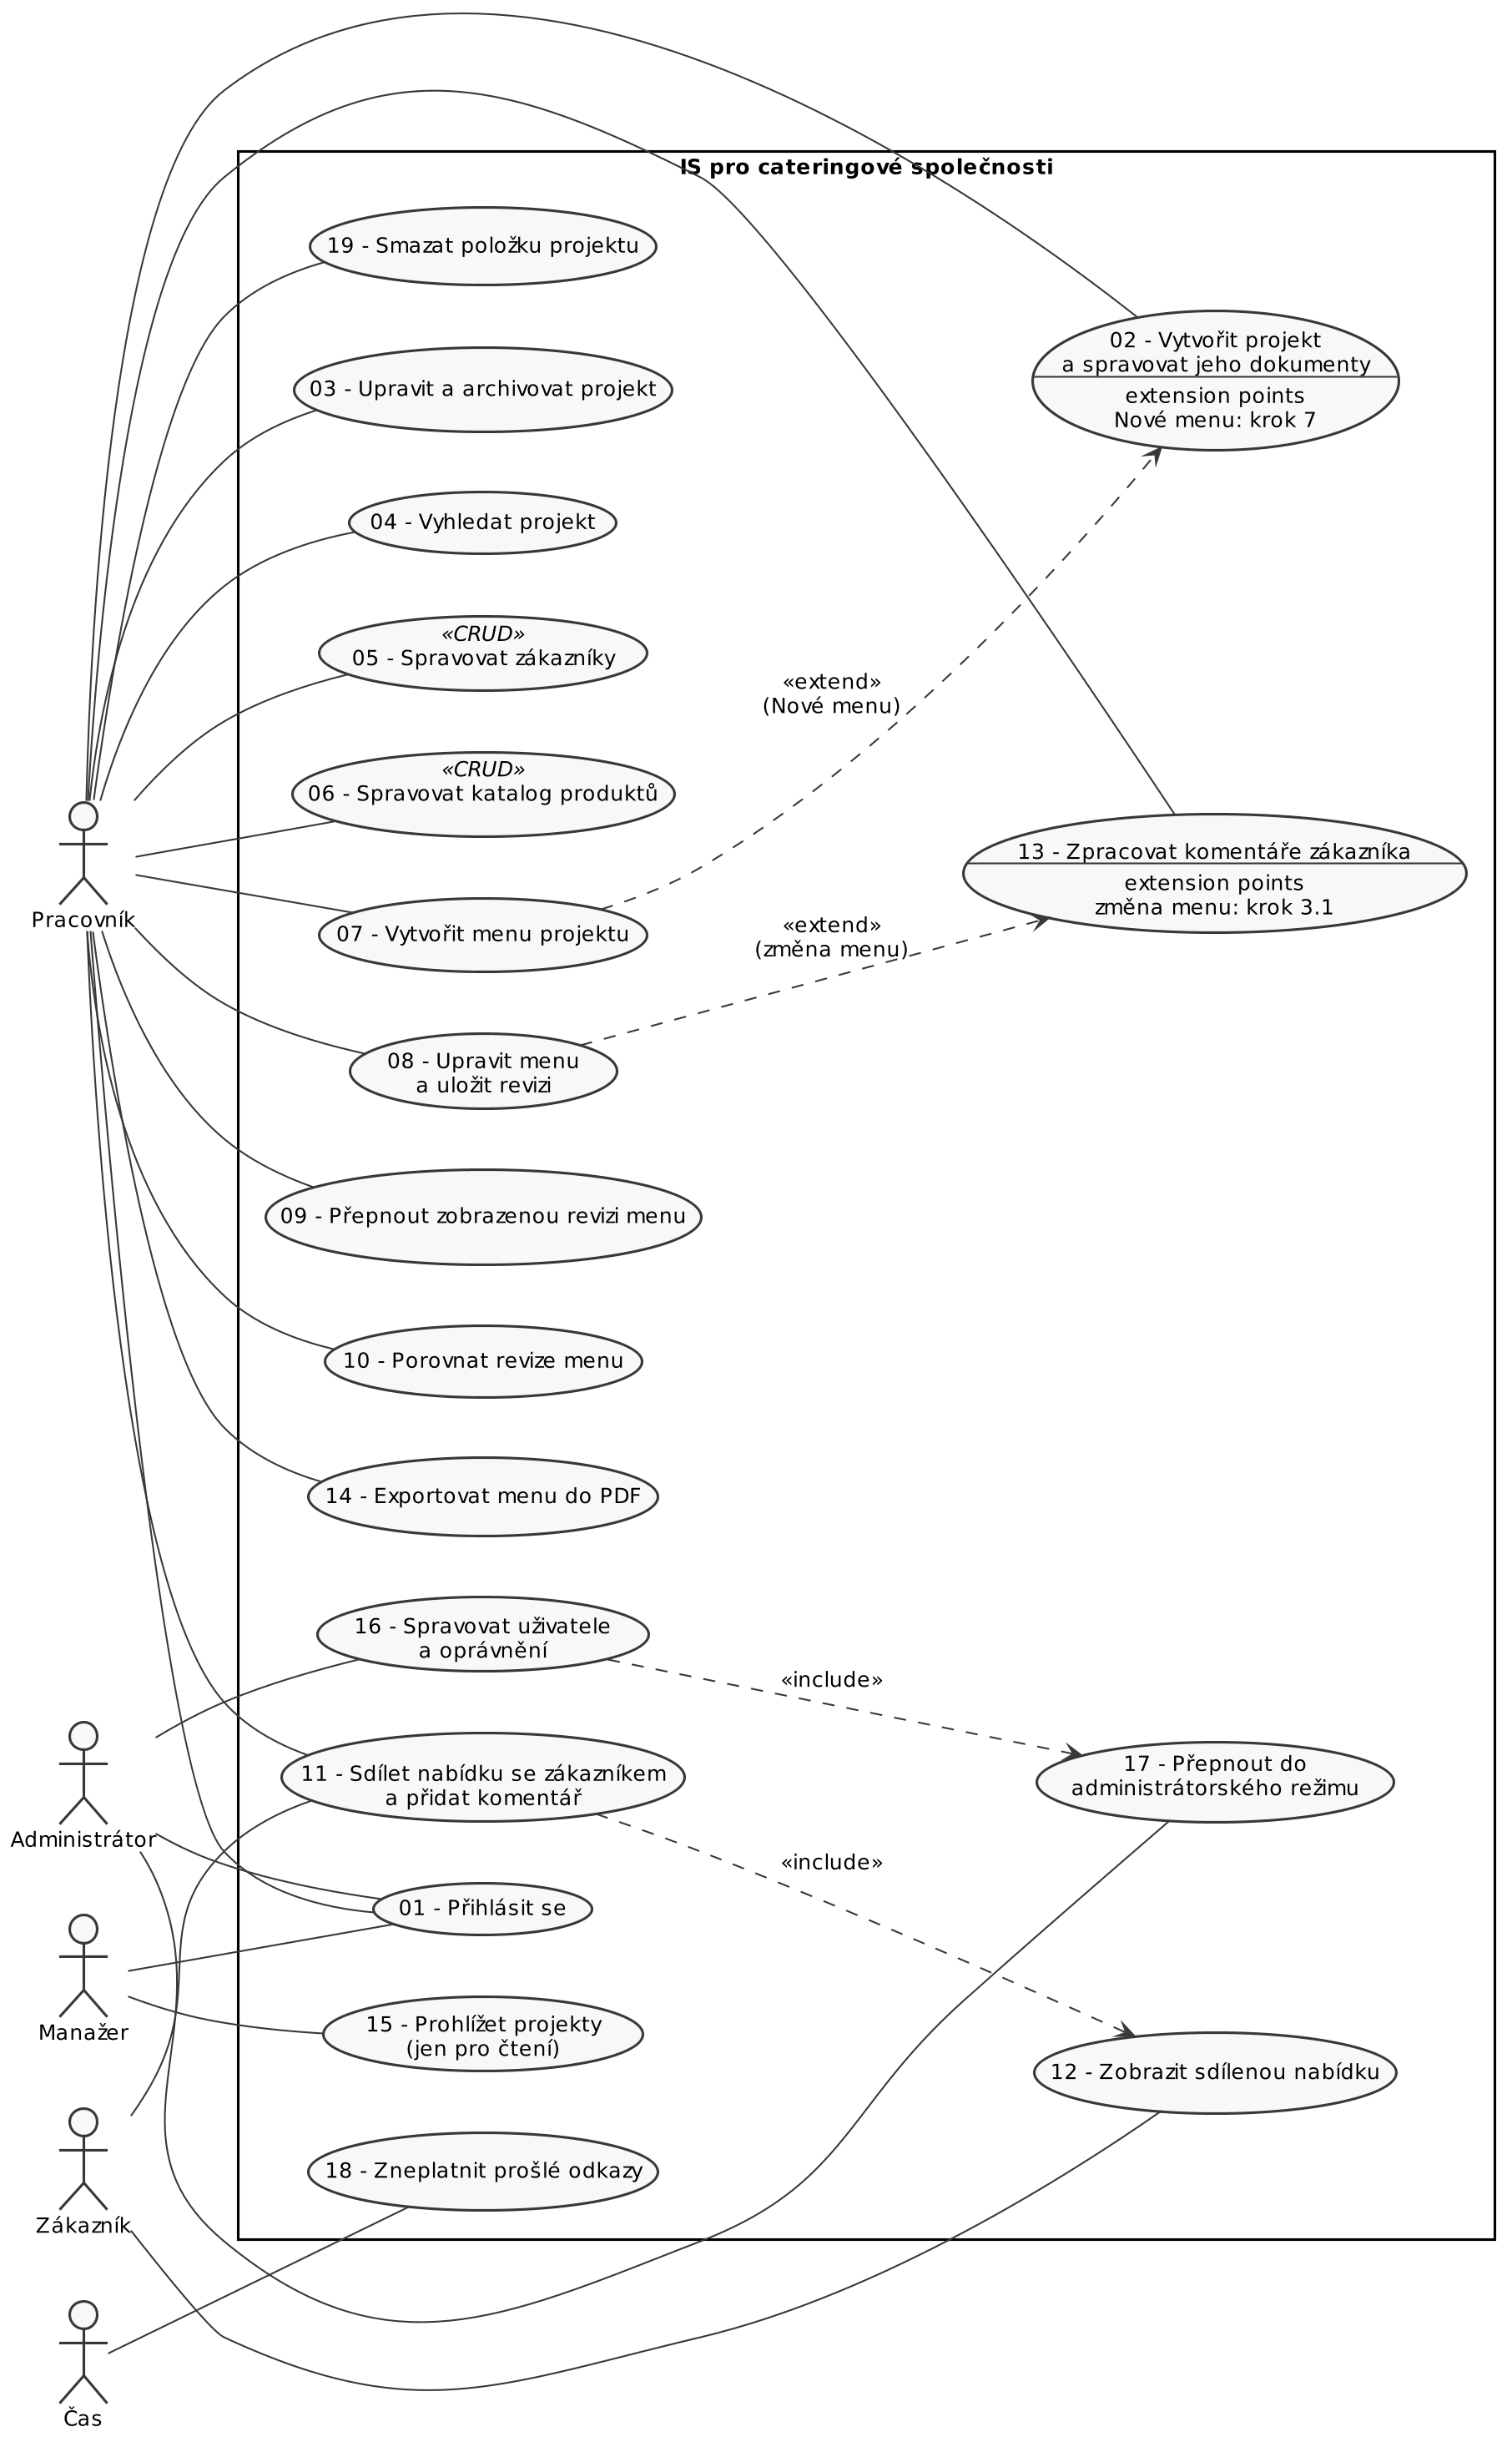
\includegraphics[width=\textwidth,height=0.82\textheight,keepaspectratio]{uc-overview.png}
  \caption{Diagram případů užití celého IS}
  \label{fig:uc}
\end{figure}
\clearpage

\subsection{Stručný popis případů užití}

\begin{description}[itemsep=1pt]
  \item[01 -- Přihlásit se:]\phantomsection\label{ucb:01} pracovník, administrátor nebo manažer se přihlásí uživatelským jménem a heslem a systém mu zpřístupní funkce podle jeho rolí. Do desktopové aplikace se přihlásí pracovník (hlavní okno) a administrátor (jen administrátorský režim, pokud nemá i roli pracovníka). Přihlášení účtu jen s rolí manažera do desktopové aplikace systém odmítne a odkáže jej na webový přehled. Po pěti neúspěšných pokusech o přihlášení ve webovém rozhraní během deseti minut systém další pokusy dočasně odmítá.
  \item[02 -- Vytvořit projekt a spravovat jeho dokumenty:]\phantomsection\label{ucb:02} pracovník založí projekt zakázky a organizuje jeho obsah do složek, menu a dokumentů, které může také stahovat na stanici (\textbf{podrobně popsán}).
  \item[03 -- Upravit a archivovat projekt:]\phantomsection\label{ucb:03} pracovník mění údaje projektu (datum, místo, počet hostů) a po skončení akce jej archivuje. Archivovaný projekt je zcela jen pro čtení (včetně nabídek, dokumentů a komentářů), dokud jej pracovník volbou \uv{Obnovit projekt} nevrátí do stavu ROZPRACOVANÝ.
  \item[04 -- Vyhledat projekt:]\phantomsection\label{ucb:04} pracovník vyhledá projekt podle názvu, zákazníka nebo data akce.
  \item[05 -- Spravovat zákazníky \guillemotleft CRUD\guillemotright:]\phantomsection\label{ucb:05} evidence zákazníků a jejich kontaktních údajů.
  \item[06 -- Spravovat katalog produktů \guillemotleft CRUD\guillemotright:]\phantomsection\label{ucb:06} evidence pokrmů a nápojů, jejich výchozích cen, jednotek, alergenů a fotografií.
  \item[07 -- Vytvořit menu projektu:]\phantomsection\label{ucb:07} pracovník založí ve složce projektu nové menu s první, zatím prázdnou revizí.
  \item[08 -- Upravit menu a uložit revizi:]\phantomsection\label{ucb:08} pracovník upravuje kategorie a položky menu a uloží je do pracovní revize, případně do nové revize, pokud byla předchozí sdílena se zákazníkem (\textbf{podrobně popsán}).
  \item[09 -- Přepnout zobrazenou revizi menu:]\phantomsection\label{ucb:09} pracovník si zobrazí libovolnou starší revizi menu.
  \item[10 -- Porovnat revize menu:]\phantomsection\label{ucb:10} systém zobrazí rozdíly mezi dvěma revizemi menu.
  \item[11 -- Sdílet nabídku se zákazníkem a přidat komentář:]\phantomsection\label{ucb:11} pracovník zpřístupní revizi menu zákazníkovi a ten k ní přidá komentář (\textbf{podrobně popsán}).
  \item[12 -- Zobrazit sdílenou nabídku:]\phantomsection\label{ucb:12} zákazník si ve webovém prohlížeči zobrazí sdílenou revizi menu.
  \item[13 -- Zpracovat komentáře zákazníka:]\phantomsection\label{ucb:13} pracovník označí komentáře jako vyřízené. Pokud komentář vyžaduje změnu menu, provede ji v rámci \ucref{08} (\textbf{podrobně popsán}).
  \item[14 -- Exportovat menu do PDF:]\phantomsection\label{ucb:14} pracovník vytvoří z revize menu dokument PDF, který se uloží mezi dokumenty projektu.
  \item[15 -- Prohlížet projekty (jen pro čtení):]\phantomsection\label{ucb:15} manažer si ve webovém rozhraní prohlíží projekty svých podřízených pracovníků, jejich menu a komentáře bez možnosti úprav. Cizí projekt systém nezobrazí. Přístup se ověřuje při každém požadavku, takže deaktivovaný manažer o něj přijde okamžitě.
  \item[16 -- Spravovat uživatele a oprávnění:]\phantomsection\label{ucb:16} administrátor vytváří a upravuje uživatelské účty a jejich role a nastavuje zapomenutá hesla (\textbf{podrobně popsán}).
  \item[17 -- Přepnout do administrátorského režimu:]\phantomsection\label{ucb:17} uživatel s rolí administrátora přepne desktopovou aplikaci do administrátorského režimu. Administrátor bez role pracovníka se do něj dostane rovnou po přihlášení, administrátor s rolí pracovníka jej přepíná tlačítkem v hlavním okně.
  \item[18 -- Zneplatnit prošlé odkazy:]\phantomsection\label{ucb:18} jednou denně systém deaktivuje sdílené odkazy, jejichž platnost skončila.
  \item[19 -- Smazat položku projektu:]\phantomsection\label{ucb:19} pracovník označí v obsahu aktivní složky jeden nebo více dokumentů, menu nebo prázdných složek a zvolí \uv{Smazat} (tlačítko s ikonou koše na červeném pozadí). Systém si vyžádá potvrzení a po něm položky odstraní.

U dokumentu smaže i soubor v úložišti dokumentů, u menu i jeho revize, komentáře a neplatné sdílené odkazy. Neprázdnou složku ani menu s aktivním sdíleným odkazem (odkaz je aktivní a jeho platnost ještě neskončila) smazat nelze. Obsahuje-li výběr takovou položku, systém nesmaže žádnou z vybraných položek a uvede důvod.
\end{description}

\subsection{Podrobný popis vybraných případů užití}

U kroků je neproporcionálním písmem uvedena operace, kterou krok vyvolá. Uživatelská rozhraní volají pouze aplikační služby, které jsou společné pro obě rozhraní (vzor Facade, viz \odkaz{sec:tech}{technická specifikace}). Pokud je u kroku uvedena metoda doménové třídy, volá ji aplikační služba.

% ---------------------------------------------------------------- UC02
\subsubsection{UC02 -- Vytvořit projekt a spravovat jeho dokumenty}\label{ucd:02}

\ucpole{Název}
Vytvořit projekt a spravovat jeho dokumenty

\ucpole{Textový popis}
Pracovník založí nový projekt pro konkrétní cateringovou zakázku. Systém k projektu automaticky vytvoří kořenovou složku.

Okno projektu má dvě části. Vlevo je strom obsahu projektu (složky, menu a dokumenty), podobný stromu souborů ve vývojovém prostředí. Vpravo je obsah aktivní složky, tedy složky vybrané ve stromu, zobrazený jako seznam souborů v běžném správci souborů.

Pracovník v projektu vytvoří podsložku a v ní nové menu, které pak v aplikaci sestaví (\ucref{08}). Do složky může také nahrát dokument ze stanice (například smlouvu nebo půdorys sálu). Jeden nebo více dokumentů aktivní složky si může stáhnout na stanici. Mazání položek popisuje \ucref{19}.

Menu se ukládá do databáze, obsah dokumentů do úložiště dokumentů a informace o nich do databáze.

\ucpole{Účastníci případu užití}
Pracovník

\ucpole{Podmínky před spuštěním}
\begin{itemize}[itemsep=0pt]
  \item Pracovník je přihlášen v desktopové aplikaci (\ucref{01}).
  \item Zákazník, pro kterého se projekt zakládá, je evidován v systému (\ucref{05}).
\end{itemize}

\ucpole{Hlavní průběh}
\begin{ucsteps}
  \item \label{uc:02:1}Pracovník v hlavním okně zvolí \uv{Nový projekt}.
  \item \label{uc:02:2}Systém zobrazí formulář projektu se seznamem zákazníků. \svc{ProjectService.findAllCustomers()}
  \item \label{uc:02:3}Pracovník vyplní název projektu, vybere zákazníka, zadá datum akce, místo konání a počet hostů a formulář potvrdí.
  \item \label{uc:02:4}Systém ověří údaje (povinné položky, datum akce není v minulosti, počet hostů je větší než 0), založí projekt ve stavu ROZPRACOVANÝ s kořenovou složkou a nastaví přihlášeného pracovníka jako odpovědného pracovníka. Zobrazí okno projektu se stromem obsahu vlevo a obsahem kořenové složky (zatím prázdným) vpravo. \svc{ProjectService.createProject()}
  \item \label{uc:02:5}Pracovník vybere ve stromu složku, otevře nabídku tlačítka \uv{Nový}, zvolí \uv{Složka} a zadá její název.
  \item \label{uc:02:6}Systém ověří název (nejvýše 100 znaků, bez lomítek \texttt{/} a \texttt{\textbackslash} a řídicích znaků, název není \uv{.} ani \uv{..}) a že ve složce neexistuje položka se stejným názvem, vytvoří podsložku, zobrazí ji ve stromu i v obsahu nadřazené složky. \svc{DocumentService.createFolder()}
  \item \label{uc:02:7}Pracovník vybere ve stromu podsložku. Systém ji nastaví jako aktivní složku a vpravo zobrazí její obsah. Pracovník v pravé části otevře nabídku tlačítka \uv{Nový}, zvolí \uv{Menu} a zadá název menu. \svc{DocumentService.listContent()}
  \item \label{uc:02:8}Systém ověří, že v aktivní složce neexistuje položka se stejným názvem. \svc{MenuService.createMenu()}
  \item \label{uc:02:9}Systém vytvoří menu s první, zatím prázdnou revizí ve stavu PRACOVNÍ, uloží je do aktivní složky a zobrazí je v jejím obsahu (\ucref{07}).
  \item \label{uc:02:10}Pracovník nové menu otevře a pokračuje jeho sestavením v \ucref{08}.
\end{ucsteps}

\ucpole{Alternativní průběh -- údaje projektu jsou neplatné}
\begin{ucalt}
  \item[4.1]\phantomsection\label{uc:02:4.1} Systém zjistí, že některý údaj chybí nebo je neplatný, a projekt nezaloží.
  \item[4.2]\phantomsection\label{uc:02:4.2} Systém zvýrazní chybná pole formuláře a zobrazí popis chyby.
  \item[4.3]\phantomsection\label{uc:02:4.3} Pracovník údaje opraví a pokračuje krokem \odkaz{uc:02:3}{3}.
\end{ucalt}

\ucpole{Alternativní průběh -- složka se stejným názvem již existuje}
\begin{ucalt}
  \item[6.1]\phantomsection\label{uc:02:6.1} Systém zjistí, že ve složce již existuje položka se stejným názvem, a podsložku nevytvoří.
  \item[6.2]\phantomsection\label{uc:02:6.2} Systém zobrazí dialog s předvyplněným volným názvem (stejně jako v kroku \odkaz{uc:02:8.1}{8.1}). Pracovník název upraví a zvolí \uv{Přejmenovat}, systém podsložku vytvoří a pokračuje krokem \odkaz{uc:02:7}{7}. Při volbě \uv{Zrušit} se podsložka nevytvoří a pokračuje se krokem \odkaz{uc:02:5}{5}.
\end{ucalt}

\ucpole{Alternativní průběh -- pracovník nahraje dokument a případně stáhne dokumenty}
\begin{ucalt}
  \item[7.1]\phantomsection\label{uc:02:7.1} Pracovník místo nabídky \uv{Nový} zvolí tlačítko \uv{Nahrát dokument}.
  \item[7.2]\phantomsection\label{uc:02:7.2} Systém zobrazí dialog pro výběr souboru na stanici.
  \item[7.3]\phantomsection\label{uc:02:7.3} Pracovník vybere soubor a potvrdí. Název dokumentu se převezme z názvu souboru.
  \item[7.4]\phantomsection\label{uc:02:7.4} Systém ověří, že soubor není větší než 20~MB. Je-li větší, zobrazí chybové hlášení s povolenou velikostí a pokračuje krokem \odkaz{uc:02:7.3}{7.3}. \svc{DocumentService.createDocument()}
  \item[7.5]\phantomsection\label{uc:02:7.5} Systém ověří, že ve složce neexistuje položka se stejným názvem. Při shodě pokračuje krokem \odkaz{uc:02:8.1}{8.1}.
  \item[7.6]\phantomsection\label{uc:02:7.6} Systém uloží obsah souboru do úložiště dokumentů a informace o dokumentu (název, typ, velikost, umístění) do databáze.
  \item[7.7]\phantomsection\label{uc:02:7.7} Systém zobrazí dokument v obsahu aktivní složky. Pokud pracovník nechce dokumenty stahovat, případ užití končí.
  \item[7.8]\phantomsection\label{uc:02:7.8} Pracovník označí v obsahu aktivní složky jeden nebo více dokumentů a zvolí \uv{Stáhnout}. Volba je dostupná jen tehdy, když jsou označeny pouze dokumenty. Menu se na stanici převádí exportem do PDF (\ucref{14}).
  \item[7.9]\phantomsection\label{uc:02:7.9} Systém zobrazí dialog pro výběr cílové složky na stanici.
  \item[7.10]\phantomsection\label{uc:02:7.10} Pracovník vybere cílovou složku a potvrdí. Při volbě \uv{Zrušit} se nic nestáhne a případ užití končí.
  \item[7.11]\phantomsection\label{uc:02:7.11} Systém načte z databáze informace o označených dokumentech, jejich obsah z úložiště dokumentů a uloží je do cílové složky. Existující soubor nikdy nepřepíše, nový uloží pod názvem s pořadovým číslem (například \uv{smlouva (2).pdf}). Dokument s neplatným uloženým názvem odmítne. \svc{DocumentService.downloadDocuments()}
  \item[7.12]\phantomsection\label{uc:02:7.12} Systém zobrazí hlášení s počtem stažených dokumentů a případ užití končí.
\end{ucalt}

\ucpole{Alternativní průběh -- položka se stejným názvem již existuje}
\begin{ucalt}
  \item[8.1]\phantomsection\label{uc:02:8.1} Systém zjistí, že v aktivní složce již existuje položka se stejným názvem, a zobrazí dialog s předvyplněným novým názvem s pořadovým číslem (například \uv{Svatební menu (2)}) a s volbami \uv{Přejmenovat} a \uv{Zrušit}.
  \item[8.2]\phantomsection\label{uc:02:8.2} Pracovník název případně upraví a zvolí \uv{Přejmenovat}.
  \item[8.3]\phantomsection\label{uc:02:8.3} Systém znovu ověří jedinečnost názvu ve složce.
  \item[8.4]\phantomsection\label{uc:02:8.4} Je-li název stále obsazen, pokračuje se krokem \odkaz{uc:02:8.1}{8.1}.
  \item[8.5]\phantomsection\label{uc:02:8.5} Je-li název volný, pokračuje se krokem \odkaz{uc:02:9}{9}, u dokumentu krokem \odkaz{uc:02:7.6}{7.6}.
\end{ucalt}
Při volbě \uv{Zrušit} v kroku \odkaz{uc:02:8.1}{8.1} se nic nevytvoří a případ užití končí.

\ucpole{Stav systému po ukončení případu užití}
\begin{itemize}[itemsep=0pt]
  \item V tabulce projektů je nový projekt ve stavu ROZPRACOVANÝ s vazbou na zákazníka a na odpovědného pracovníka.
  \item V tabulce obsahu projektu jsou nové záznamy: kořenová složka, podsložka (typ FOLDER) a menu (typ MENU) s odkazem na nadřazenou složku.
  \item V tabulce revizí menu je první revize nového menu ve stavu PRACOVNÍ, zatím bez kategorií a položek.
  \item Při alternativním průběhu \odkaz{uc:02:7.1}{7.1} je místo menu v tabulce obsahu projektu dokument (typ DOCUMENT) a v úložišti dokumentů existuje soubor s jeho obsahem pod klíčem uloženým u dokumentu v databázi.
  \item Stažení dokumentů (kroky \odkaz{uc:02:7.8}{7.8} až \odkaz{uc:02:7.12}{7.12}) obsah úložiště ani databáze nemění.
\end{itemize}

\clearpage
\begin{figure}[H]
  \centering
  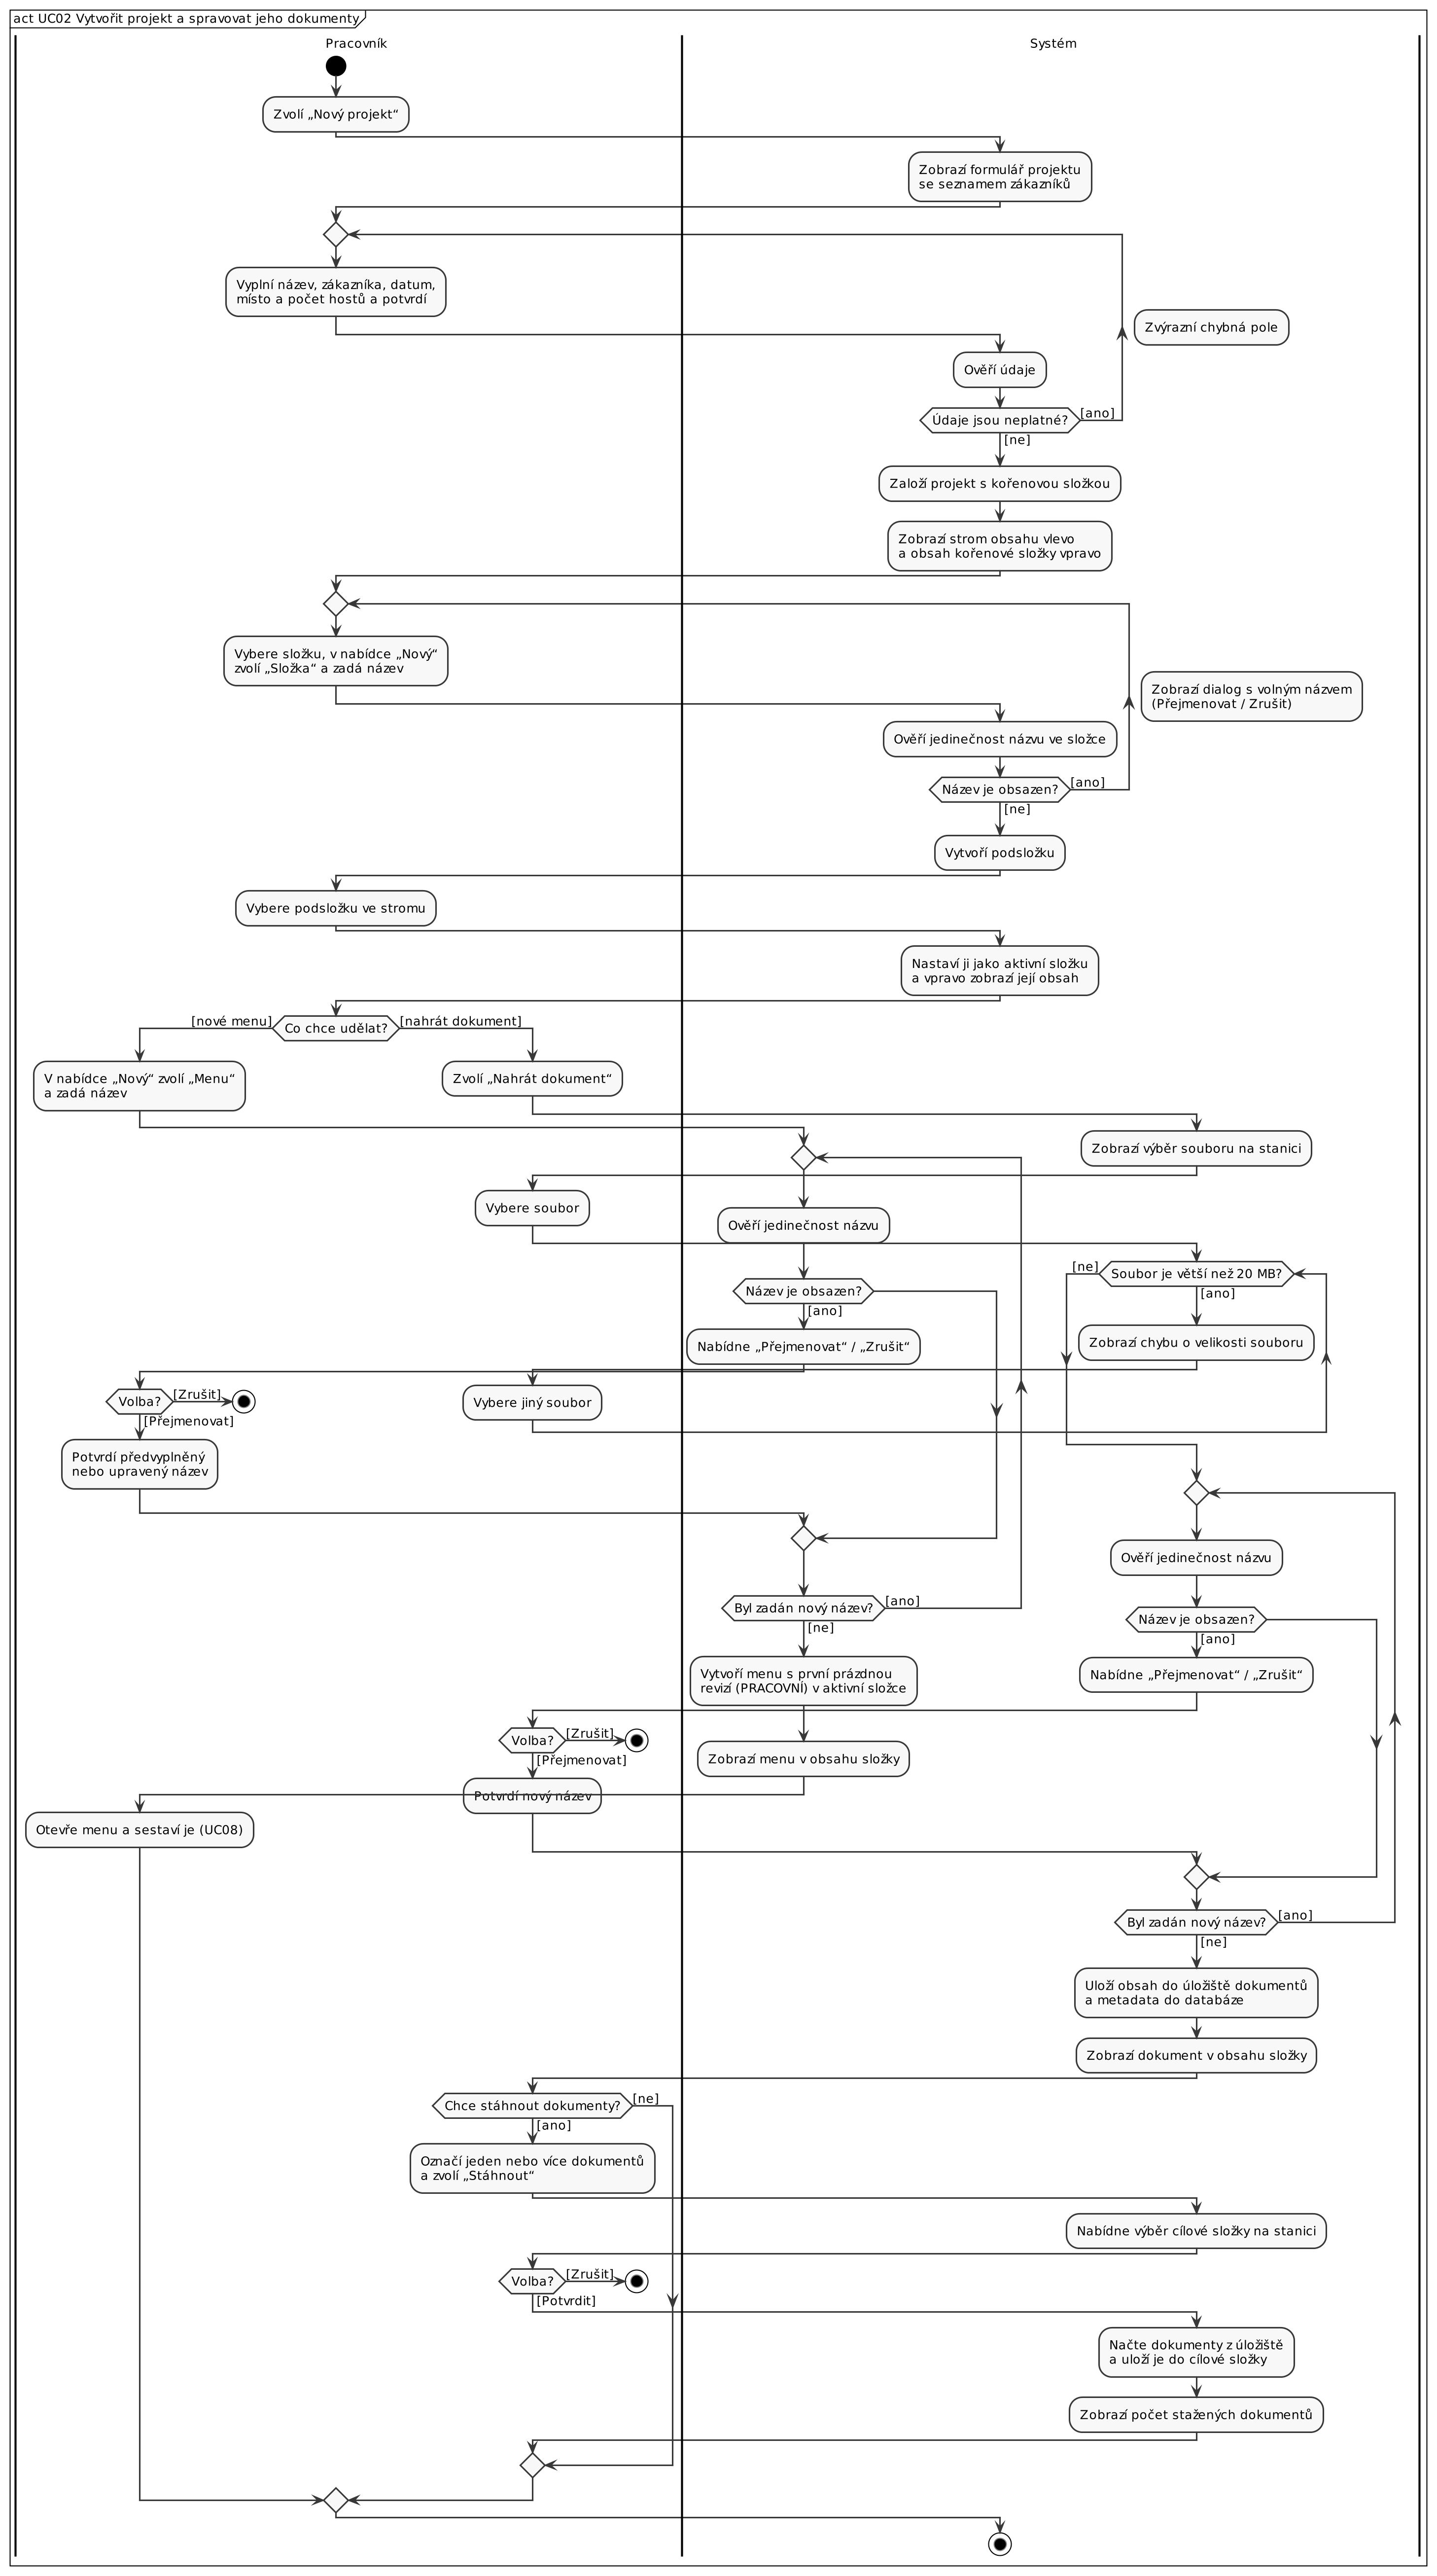
\includegraphics[width=\textwidth,height=0.8\textheight,keepaspectratio]{act-uc02.png}
  \caption{Diagram aktivit UC02 -- Vytvořit projekt a spravovat jeho dokumenty}
\end{figure}
\clearpage

% ---------------------------------------------------------------- UC08
\subsubsection{UC08 -- Upravit menu a uložit revizi}\label{ucd:08}

\ucpole{Název}
Upravit menu a uložit revizi

\ucpole{Textový popis}
Pracovník upraví menu projektu: přidává a odebírá kategorie a položky z katalogu produktů a mění jejich množství a cenu. Systém průběžně přepočítává cenu menu.

Pracovní revize (stav PRACOVNÍ) se při uložení přepíše a její číslo se nemění. Revizi, která již byla sdílena se zákazníkem (stav SDÍLENÁ), nelze měnit. Úpravy sdílené revize se proto uloží jako nová revize s číslem o jedna vyšším, takže verze, kterou zákazník viděl, zůstane zachována. Pracovní může být vždy jen nejnovější revize menu, proto pracovní kopii nelze vytvořit, dokud je nejnovější revize pracovní.

Zjednodušení: revize ukládá u každé položky množství a jednotkovou cenu, ale název produktu, alergeny a sazbu DPH se čtou vždy z aktuálního katalogu produktů. Sdílená revize proto zobrazuje aktuální názvy a alergeny z katalogu, i když se po sdílení změnily.

\ucpole{Účastníci případu užití}
Pracovník

\ucpole{Podmínky před spuštěním}
\begin{itemize}[itemsep=0pt]
  \item Pracovník je přihlášen v desktopové aplikaci (\ucref{01}).
  \item Projekt obsahuje menu s alespoň jednou revizí (\ucref{02}, \ucref{07}).
  \item V katalogu produktů existují produkty (\ucref{06}).
\end{itemize}

\ucpole{Hlavní průběh}
\begin{ucsteps}
  \item \label{uc:08:1}Pracovník otevře projekt a vybere v něm menu.
  \item \label{uc:08:2}Systém načte nejnovější revizi menu a zobrazí její kategorie a položky. Revize je ve stavu PRACOVNÍ, a proto je editace povolena. \svc{MenuService.openLatestRevision()}
  \item \label{uc:08:3}Pracovník přidá kategorii, vybere do ní produkty z katalogu a upraví jejich množství a jednotkovou cenu. \svc{MenuService.findProducts()}
  \item \label{uc:08:4}Systém po každé změně přepočítá cenu kategorií, celkovou cenu menu a cenu na jednoho hosta. \svc{MenuEditor.execute()}, \svc{ChangeItemCommand}, \svc{MenuRevision.totalPrice()}, \svc{MenuRevision.pricePerGuest()}
  \item \label{uc:08:5}Pracovník zvolí \uv{Uložit revizi} a zadá poznámku ke změně.
  \item \label{uc:08:6}Systém zkontroluje menu: obsahuje alespoň jednu kategorii, název kategorie má nejvýše 60 znaků, každá položka má vyplněné množství větší než 0 (nejvýše dvě desetinná místa, méně než 1~000~000) a vyplněnou cenu alespoň 0 a méně než 100~000~000, poznámka k položce má nejvýše 200 znaků a žádný produkt není v jedné kategorii dvakrát. Poznámka ke změně má nejvýše 500 znaků. \svc{MenuService.saveRevision()}, \svc{MenuRevision.validate()}
  \item \label{uc:08:7}Systém v jedné databázové transakci přepíše pracovní revizi včetně jejích kategorií a položek. Číslo revize se nemění. Starší revize zůstanou beze změny.
  \item \label{uc:08:8}Systém zobrazí potvrzení s číslem uložené revize a aktualizuje seznam revizí menu.
\end{ucsteps}

\ucpole{Alternativní průběh -- nejnovější revize je již sdílena se zákazníkem}
\begin{ucalt}
  \item[2.1]\phantomsection\label{uc:08:2.1} Systém zjistí, že nejnovější revize menu je ve stavu SDÍLENÁ.
  \item[2.2]\phantomsection\label{uc:08:2.2} Systém zobrazí revizi jen pro čtení s upozorněním, že sdílenou revizi nelze měnit, a zakáže editační prvky.
  \item[2.3]\phantomsection\label{uc:08:2.3} Pracovník zvolí \uv{Vytvořit pracovní kopii}.
  \item[2.4]\phantomsection\label{uc:08:2.4} Systém vytvoří z otevřené revize pracovní kopii (zatím neuloženou) a povolí editaci. \svc{MenuService.createWorkingCopy()}
  \item[2.5]\phantomsection\label{uc:08:2.5} Pokračuje se krokem \odkaz{uc:08:3}{3}. V kroku \odkaz{uc:08:7}{7} systém pracovní kopii uloží jako novou revizi s číslem o jedna vyšším ve stavu PRACOVNÍ. Sdílená revize i odkaz na ni zůstanou beze změny.
\end{ucalt}

\ucpole{Alternativní průběh -- nejnovější revize je již pracovní}
\begin{ucalt}
  \item[2.6]\phantomsection\label{uc:08:2.6} Pracovník má otevřenou starší sdílenou revizi (\ucref{09}), zatímco nejnovější revize menu je ve stavu PRACOVNÍ, a v kroku \odkaz{uc:08:2.3}{2.3} zvolí \uv{Vytvořit pracovní kopii}.
  \item[2.7]\phantomsection\label{uc:08:2.7} Systém zjistí, že nejnovější revize menu je ve stavu PRACOVNÍ, a pracovní kopii nevytvoří.
  \item[2.8]\phantomsection\label{uc:08:2.8} Systém zobrazí zprávu \uv{Nejnovější revize je pracovní. Upravte ji, nebo ji nejprve sdílejte.} a ponechá zobrazenou sdílenou revizi jen pro čtení.
  \item[2.9]\phantomsection\label{uc:08:2.9} Pracovník v seznamu revizí zvolí nejnovější (pracovní) revizi. Systém ji zobrazí s povolenou editací.
  \item[2.10]\phantomsection\label{uc:08:2.10} Pokračuje se krokem \odkaz{uc:08:3}{3}.
\end{ucalt}

\ucpole{Alternativní průběh -- menu obsahuje chyby}
\begin{ucalt}
  \item[6.1]\phantomsection\label{uc:08:6.1} Systém zjistí, že menu nesplňuje některou z kontrol.
  \item[6.2]\phantomsection\label{uc:08:6.2} Systém nic neuloží, zvýrazní chybné položky a zobrazí popis chyby.
  \item[6.3]\phantomsection\label{uc:08:6.3} Pracovník chyby opraví (kroky \odkaz{uc:08:3}{3} a \odkaz{uc:08:4}{4}) a pokračuje krokem \odkaz{uc:08:5}{5}.
\end{ucalt}

\ucpole{Alternativní průběh -- revizi mezitím změnil jiný pracovník}
\begin{ucalt}
  \item[7.1]\phantomsection\label{uc:08:7.1} Systém při ukládání zjistí, že otevřená revize byla mezitím sdílena se zákazníkem nebo že mezitím vznikla novější revize menu.
  \item[7.2]\phantomsection\label{uc:08:7.2} Systém nic neuloží a zobrazí zprávu, že menu mezitím změnil jiný pracovník.
  \item[7.3]\phantomsection\label{uc:08:7.3} Systém načte nejnovější revizi menu a pokračuje se krokem \odkaz{uc:08:2}{2}.
\end{ucalt}

\ucpole{Stav systému po ukončení případu užití}
\begin{itemize}[itemsep=0pt]
  \item Pracovní revize má v tabulce revizí menu novou poznámku a čas posledního uložení. Její kategorie a položky v tabulkách kategorií a položek odpovídají uloženému stavu.
  \item Při alternativním průběhu \odkaz{uc:08:2.1}{2.1} je v tabulce revizí nová revize s číslem o jedna vyšším ve stavu PRACOVNÍ s vlastními kategoriemi a položkami.
  \item Záznamy předchozích revizí (včetně sdílené revize a jejích odkazů) se nezměnily.
\end{itemize}

\clearpage
\begin{figure}[H]
  \centering
  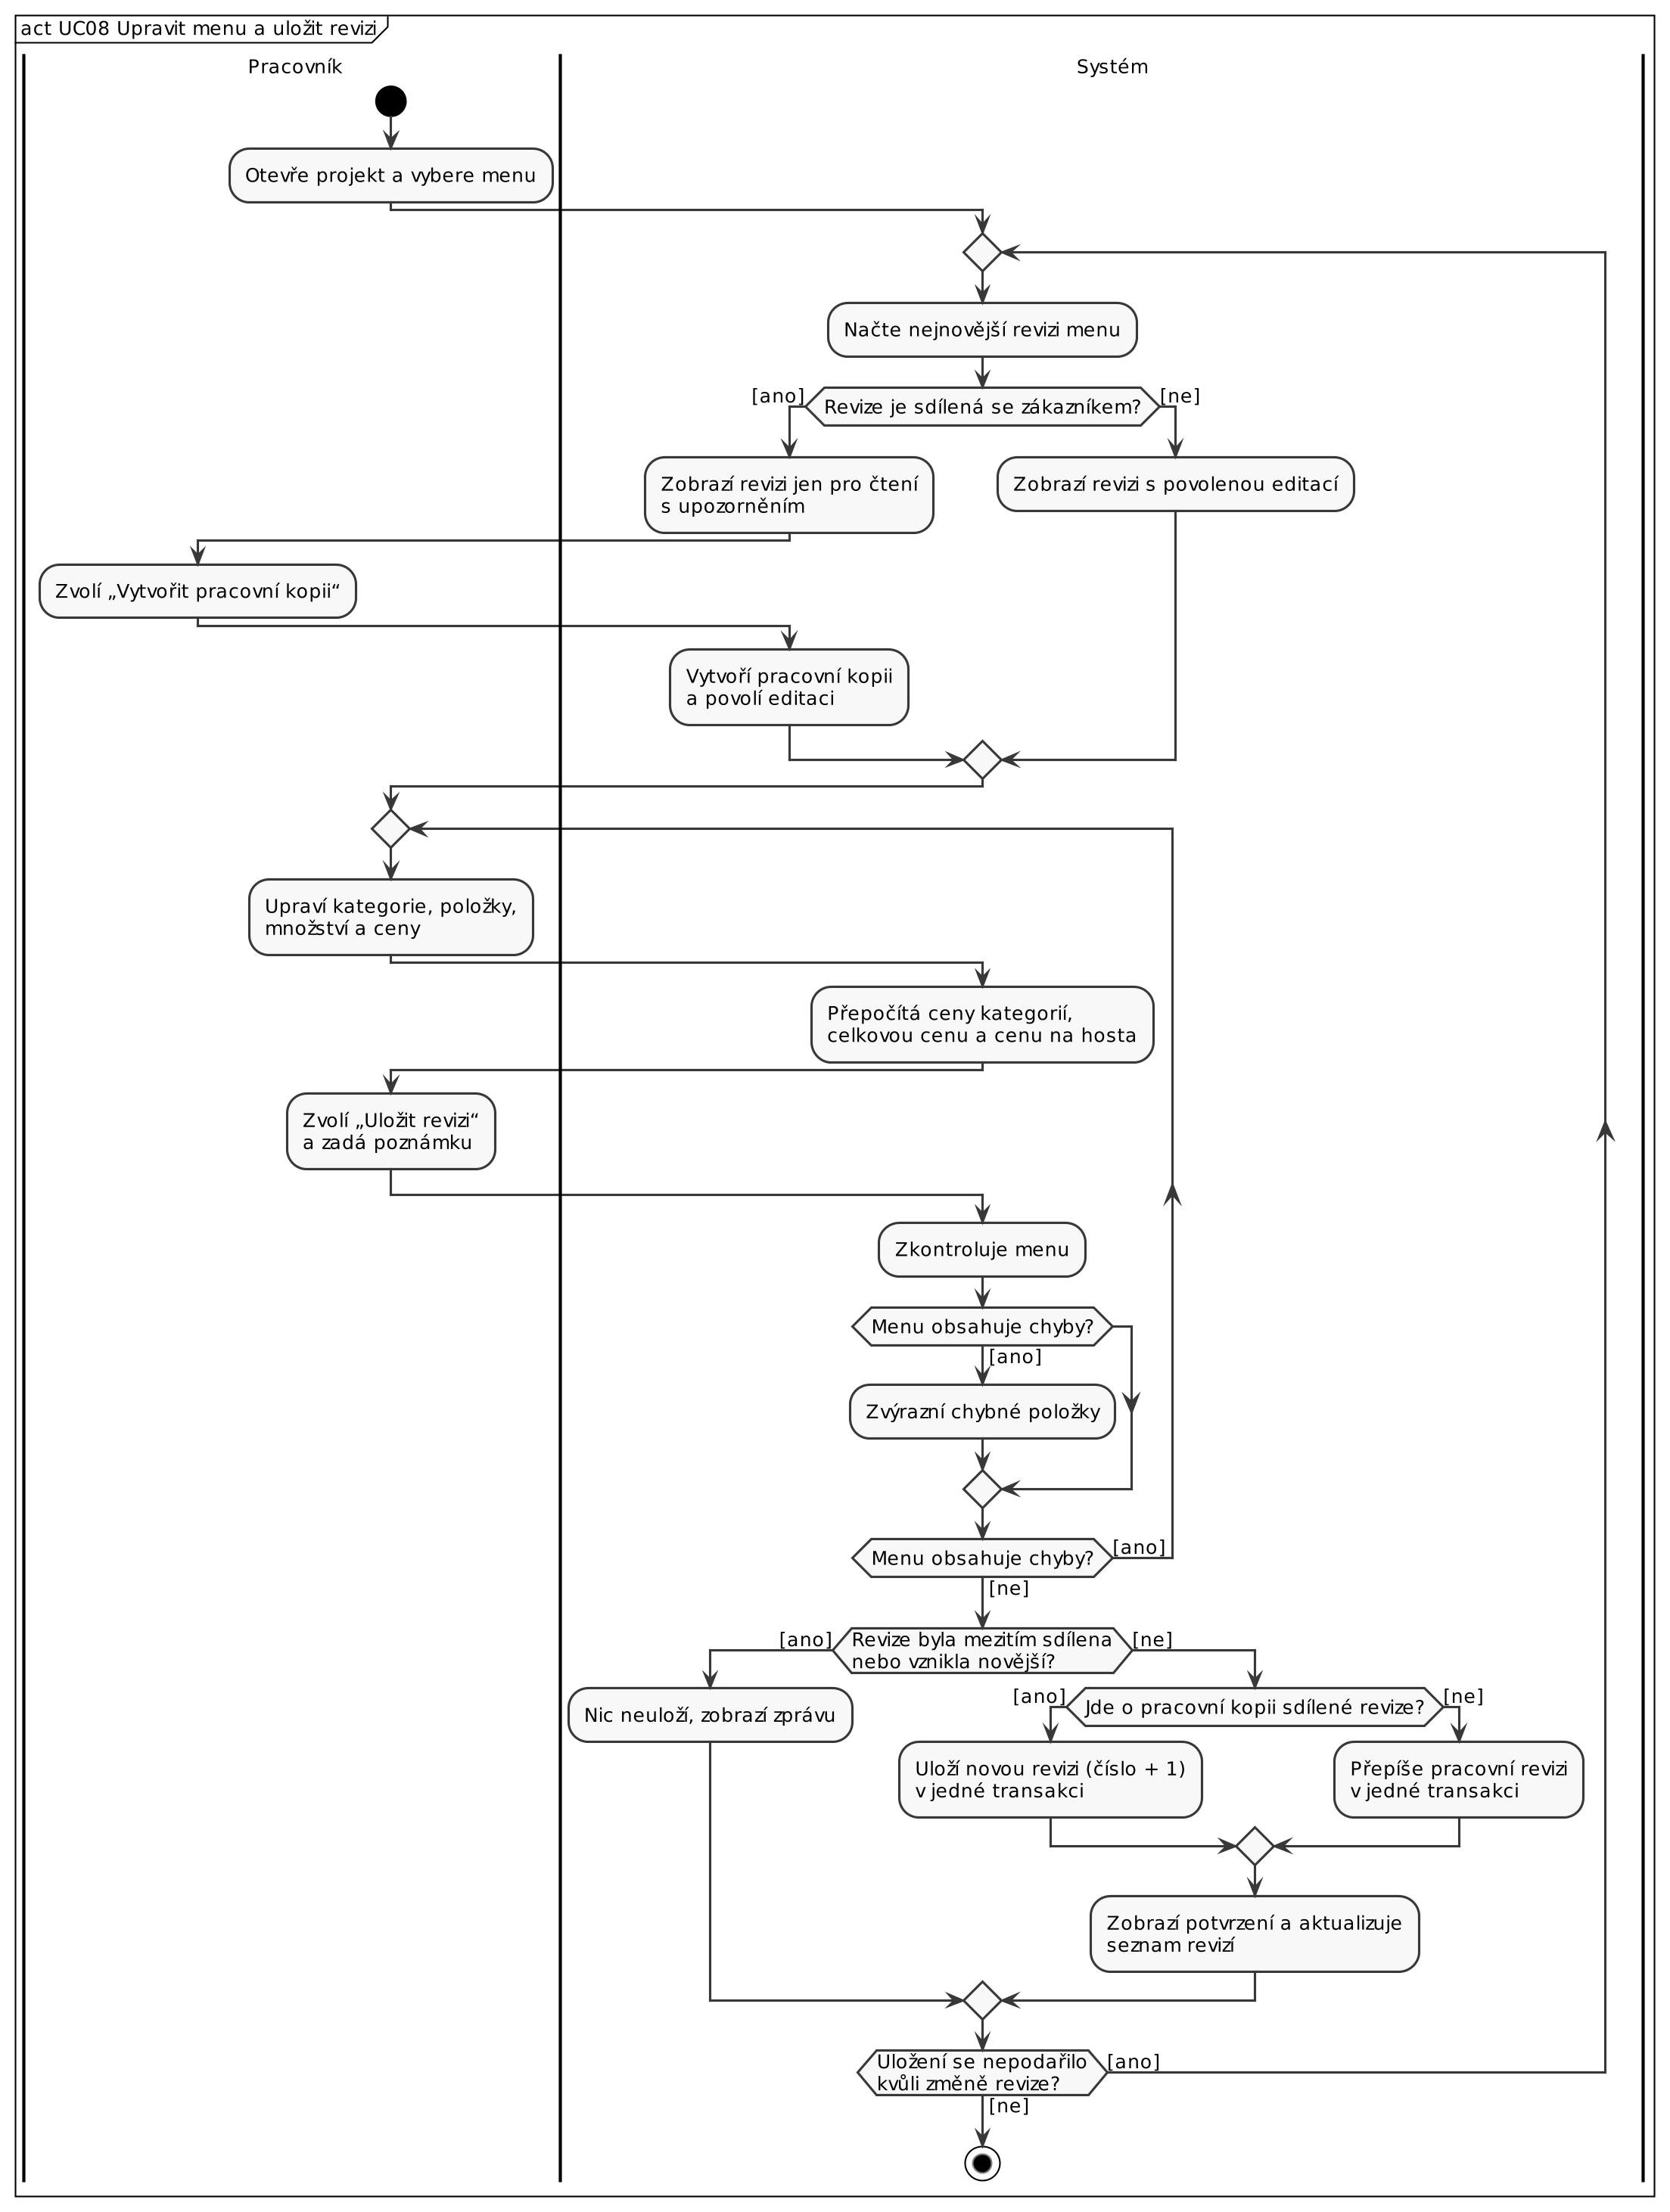
\includegraphics[width=\textwidth,height=0.75\textheight,keepaspectratio]{act-uc08.png}
  \caption{Diagram aktivit UC08 -- Upravit menu a uložit revizi}
\end{figure}
\clearpage

% ---------------------------------------------------------------- UC11
\subsubsection{UC11 -- Sdílet nabídku se zákazníkem a přidat komentář}\label{ucd:11}

\ucpole{Název}
Sdílet nabídku se zákazníkem a přidat komentář

\ucpole{Textový popis}
Pracovník zpřístupní vybranou revizi menu zákazníkovi. Systém revizi uzamkne (stav SDÍLENÁ), zneplatní starší odkazy na totéž menu a vytvoří nový odkaz s omezenou platností, který zobrazí i jako QR kód. Zákazník odkaz otevře ve webovém prohlížeči, prohlédne si nabídku a přidá k ní komentář. Komentář se uloží k revizi a pracovník jej uvidí v desktopové aplikaci.

\ucpole{Účastníci případu užití}
Pracovník, Zákazník

\ucpole{Podmínky před spuštěním}
\begin{itemize}[itemsep=0pt]
  \item Pracovník je přihlášen v desktopové aplikaci (\ucref{01}).
  \item Menu projektu má revizi s alespoň jednou kategorií, která prošla kontrolou při uložení (\ucref{08}, krok \odkaz{uc:08:6}{6}).
  \item Webové rozhraní systému je spuštěno a dostupné pro zákazníka.
\end{itemize}

\ucpole{Hlavní průběh}
\begin{ucsteps}
  \item \label{uc:11:1}Pracovník otevře menu, vybere revizi a zvolí \uv{Sdílet se zákazníkem}. Volba je dostupná jen u revize, která obsahuje alespoň jednu kategorii.
  \item \label{uc:11:2}Systém označí revizi jako SDÍLENOU, zneplatní předchozí aktivní odkazy na toto menu a vytvoří nový odkaz s náhodným identifikátorem a platností 14 dní. \svc{SharingService.shareRevision()}, \svc{MenuRevision.validate()}
  \item \label{uc:11:3}Systém zobrazí dialog s odkazem a QR kódem. Pracovník odkaz zkopíruje a předá zákazníkovi (například e-mailem mimo systém).
  \item \label{uc:11:4}Zákazník otevře odkaz ve webovém prohlížeči.
  \item \label{uc:11:5}Systém ověří, že odkaz existuje, je aktivní a není prošlý, a zobrazí sdílenou revizi menu s kategoriemi, položkami, cenami, alergeny a dosavadními komentáři (\ucref{12}). \svc{SharingService.openSharedMenu()}
  \item \label{uc:11:6}Zákazník napíše komentář k celému menu nebo vybere konkrétní položku, vyplní své jméno a komentář odešle.
  \item \label{uc:11:7}Systém ověří komentář (jméno i text jsou vyplněny, text má nejvýše 2000 znaků) a uloží jej k revizi jako nevyřízený. \svc{SharingService.addComment()}
  \item \label{uc:11:8}Systém zobrazí zákazníkovi potvrzení a komentář v seznamu komentářů. Pracovník komentář uvidí u revize v desktopové aplikaci.
\end{ucsteps}

\ucpole{Alternativní průběh -- revizi mezitím změnil jiný pracovník}
\begin{ucalt}
  \item[2.1]\phantomsection\label{uc:11:2.1} Systém při sdílení zjistí, že otevřená pracovní revize byla mezitím jiným pracovníkem přepsána nebo že vznikla novější revize menu.
  \item[2.2]\phantomsection\label{uc:11:2.2} Systém revizi nesdílí a stávající odkazy ponechá beze změny.
  \item[2.3]\phantomsection\label{uc:11:2.3} Systém zobrazí zprávu, že menu mezitím změnil jiný pracovník.
  \item[2.4]\phantomsection\label{uc:11:2.4} Systém načte nejnovější revizi menu.
  \item[2.5]\phantomsection\label{uc:11:2.5} Pracovník nejnovější revizi zkontroluje a pokračuje krokem \odkaz{uc:11:1}{1}.
\end{ucalt}

\ucpole{Alternativní průběh -- odkaz je prošlý nebo nahrazený novějším}
\begin{ucalt}
  \item[5.1]\phantomsection\label{uc:11:5.1} Systém zjistí, že platnost odkazu skončila nebo že odkaz byl zneplatněn novějším sdílením téhož menu. Pokud odkaz vůbec neexistuje, systém zobrazí zprávu \uv{Odkaz není platný, kontaktujte pracovníka} a případ užití končí.
  \item[5.2]\phantomsection\label{uc:11:5.2} Systém původní revizi nezobrazí a zobrazí zprávu \uv{Odkaz již není platný}.
  \item[5.3]\phantomsection\label{uc:11:5.3} Systém vyhledá aktivní a neprošlý odkaz téhož menu. Pokud existuje, nabídne zobrazení aktuální nabídky. Jinak zákazníkovi doporučí kontaktovat pracovníka a případ užití končí.
  \item[5.4]\phantomsection\label{uc:11:5.4} Zákazník zvolí \uv{Zobrazit aktuální nabídku}.
  \item[5.5]\phantomsection\label{uc:11:5.5} Systém zobrazí revizi, na kterou vede nalezený odkaz, s jejími komentáři.
  \item[5.6]\phantomsection\label{uc:11:5.6} Pokračuje se krokem \odkaz{uc:11:6}{6}.
\end{ucalt}

\ucpole{Alternativní průběh -- komentář je neplatný}
\begin{ucalt}
  \item[7.1]\phantomsection\label{uc:11:7.1} Systém zjistí, že jméno nebo text komentáře chybí nebo že text má více než 2000 znaků.
  \item[7.2]\phantomsection\label{uc:11:7.2} Systém komentář neuloží a zvýrazní chybná pole.
  \item[7.3]\phantomsection\label{uc:11:7.3} Zákazník údaje opraví a pokračuje krokem \odkaz{uc:11:6}{6}.
\end{ucalt}
Pokud mezitím skončila platnost odkazu, systém komentář v kroku \odkaz{uc:11:7}{7} neuloží a pokračuje krokem \odkaz{uc:11:5.1}{5.1}.

\ucpole{Stav systému po ukončení případu užití}
\begin{itemize}[itemsep=0pt]
  \item Revize menu je v tabulce revizí ve stavu SDÍLENÁ.
  \item V tabulce odkazů je nový aktivní odkaz na revizi s datem platnosti. Dřívější odkazy na stejné menu jsou neaktivní.
  \item V tabulce komentářů je nový nevyřízený komentář s jménem zákazníka, textem, datem a vazbou na revizi (případně na položku menu).
\end{itemize}

\clearpage
\begin{figure}[H]
  \centering
  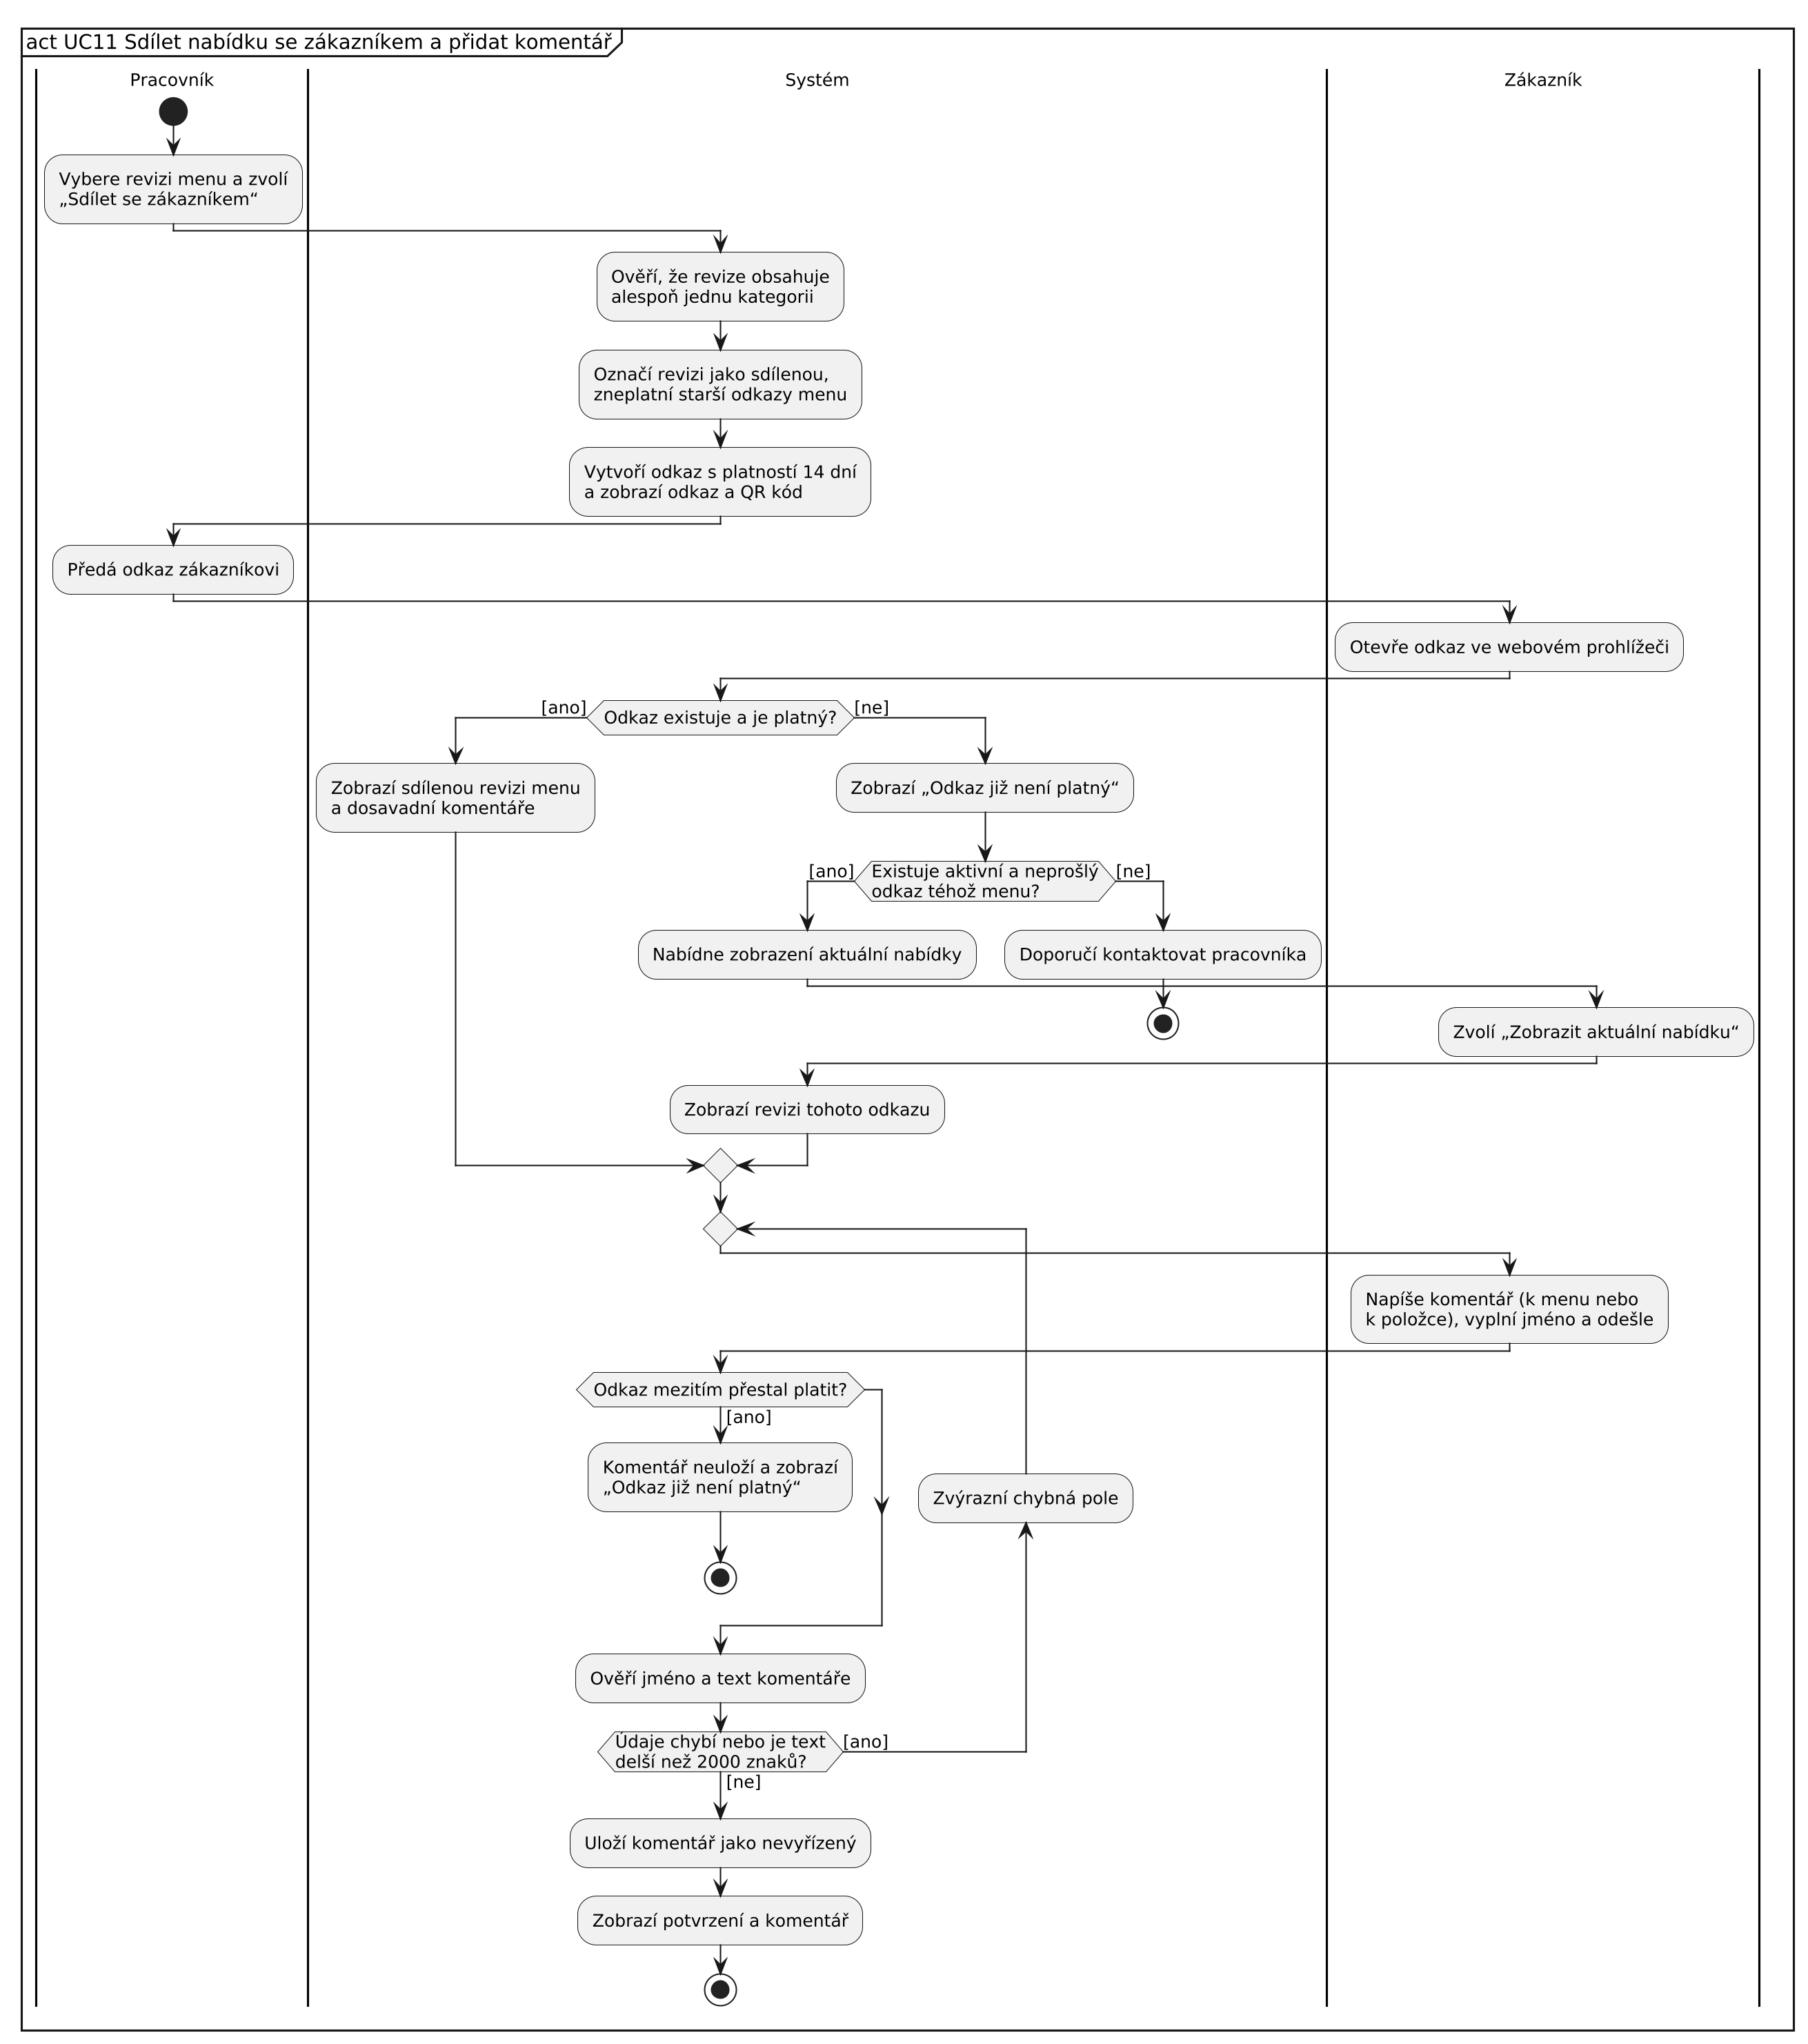
\includegraphics[width=\textwidth,height=0.8\textheight,keepaspectratio]{act-uc11.png}
  \caption{Diagram aktivit UC11 -- Sdílet nabídku se zákazníkem a přidat komentář}
\end{figure}
\clearpage

% ---------------------------------------------------------------- UC13
\subsubsection{UC13 -- Zpracovat komentáře zákazníka}\label{ucd:13}

\ucpole{Název}
Zpracovat komentáře zákazníka

\ucpole{Textový popis}
Pracovník projde komentáře, které zákazník přidal ke sdílené revizi menu. Ke každému nevyřízenému komentáři zapíše poznámku, jak byl vyřízen, a označí jej jako vyřízený. Systém u komentáře uloží, kdo a kdy jej vyřídil. Pokud komentář vyžaduje změnu menu, pracovník ji provede v rámci \ucref{08} a komentář vyřídí s odkazem na číslo uložené revize.

\ucpole{Účastníci případu užití}
Pracovník

\ucpole{Podmínky před spuštěním}
\begin{itemize}[itemsep=0pt]
  \item Pracovník je přihlášen v desktopové aplikaci (\ucref{01}).
  \item Revize menu byla sdílena se zákazníkem a zákazník k ní přidal alespoň jeden komentář (\ucref{11}).
\end{itemize}

\ucpole{Hlavní průběh}
\begin{ucsteps}
  \item \label{uc:13:1}Pracovník v editoru menu otevře sdílenou revizi a zvolí tlačítko s komentáři a počtem nevyřízených, například \uv{Komentáře k rev. 2 (3 nevyřízených)}.
  \item \label{uc:13:2}Systém načte komentáře revize a zobrazí je seřazené tak, že nevyřízené jsou nahoře. U každého zobrazí jméno zákazníka, datum, text a položku menu, které se týká. \svc{SharingService.listComments()}
  \item \label{uc:13:3}Pracovník vybere nevyřízený komentář, zapíše poznámku k vyřízení (pole dovolí zapsat nejvýše 200 znaků) a zvolí \uv{Označit jako vyřízený}.
  \item \label{uc:13:4}Systém ověří, že komentář je stále nevyřízený a poznámka má nejvýše 200 znaků. \svc{SharingService.resolveComment()}
  \item \label{uc:13:5}Systém uloží u komentáře příznak vyřízený, poznámku, přihlášeného pracovníka jako autora vyřízení a datum vyřízení. \svc{Comment.resolve()}
  \item \label{uc:13:6}Systém přesune komentář mezi vyřízené a v editoru menu aktualizuje počet nevyřízených komentářů.
  \item \label{uc:13:7}Pracovník opakuje kroky \odkaz{uc:13:3}{3} až \odkaz{uc:13:6}{6} pro další komentáře. Když nezůstane žádný nevyřízený komentář, systém zobrazí zprávu \uv{Všechny komentáře jsou vyřízeny}.
\end{ucsteps}

\ucpole{Alternativní průběh -- komentář vyžaduje změnu menu}
\begin{ucalt}
  \item[3.1]\phantomsection\label{uc:13:3.1} Pracovník u vybraného komentáře zvolí \uv{Upravit menu podle komentáře}.
  \item[3.2]\phantomsection\label{uc:13:3.2} Systém otevře v editoru nejnovější revizi menu (\ucref{08}, krok \odkaz{uc:08:2}{2}, u sdílené revize kroky \odkaz{uc:08:2.1}{2.1} až \odkaz{uc:08:2.4}{2.4}) a zvýrazní položku se stejným produktem, jakého se komentář týká. Úpravy podle dřívějších komentářů tak zůstanou zachovány.
  \item[3.3]\phantomsection\label{uc:13:3.3} Pracovník upraví menu a uloží revizi (\ucref{08}, kroky \odkaz{uc:08:3}{3} až \odkaz{uc:08:7}{7}).
  \item[3.4]\phantomsection\label{uc:13:3.4} Systém se vrátí ke zpracování komentářů a předvyplní poznámku k vyřízení textem \uv{Upraveno v revizi č.~N}.
  \item[3.5]\phantomsection\label{uc:13:3.5} Pracovník poznámku případně doplní a zvolí \uv{Označit jako vyřízený}. Pokračuje se krokem \odkaz{uc:13:4}{4}.
\end{ucalt}

\ucpole{Alternativní průběh -- komentář mezitím vyřídil jiný pracovník}
\begin{ucalt}
  \item[4.1]\phantomsection\label{uc:13:4.1} Systém zjistí, že komentář je již označen jako vyřízený.
  \item[4.2]\phantomsection\label{uc:13:4.2} Systém nic neuloží a zobrazí zprávu, kdo a kdy komentář vyřídil.
  \item[4.3]\phantomsection\label{uc:13:4.3} Systém znovu načte komentáře revize a zobrazí aktuální stav.
  \item[4.4]\phantomsection\label{uc:13:4.4} Pracovník vybere další nevyřízený komentář a pokračuje krokem \odkaz{uc:13:3}{3}.
  \item[4.5]\phantomsection\label{uc:13:4.5} Pokud žádný nevyřízený komentář nezůstal, systém zobrazí zprávu \uv{Všechny komentáře jsou vyřízeny} a případ užití končí.
\end{ucalt}

\ucpole{Alternativní průběh -- pracovník ukončí zpracování dříve}
\begin{ucalt}
  \item[7.1]\phantomsection\label{uc:13:7.1} Pracovník místo dalšího komentáře zavře zpracování komentářů, i když zbývají nevyřízené.
  \item[7.2]\phantomsection\label{uc:13:7.2} Systém nevyřízené komentáře ponechá beze změny a v editoru menu zobrazí jejich počet. Případ užití končí.
\end{ucalt}

\ucpole{Stav systému po ukončení případu užití}
\begin{itemize}[itemsep=0pt]
  \item V tabulce komentářů má zpracovaný komentář příznak vyřízený, poznámku k vyřízení, vazbu na pracovníka, který jej vyřídil, a datum vyřízení.
  \item Komentáře, které pracovník nezpracoval, zůstaly beze změny.
  \item Při alternativním průběhu \odkaz{uc:13:3.1}{3.1} je navíc uložena pracovní nebo nová revize menu (\ucref{08}) a poznámka komentáře obsahuje její číslo.
\end{itemize}

\clearpage
\begin{figure}[H]
  \centering
  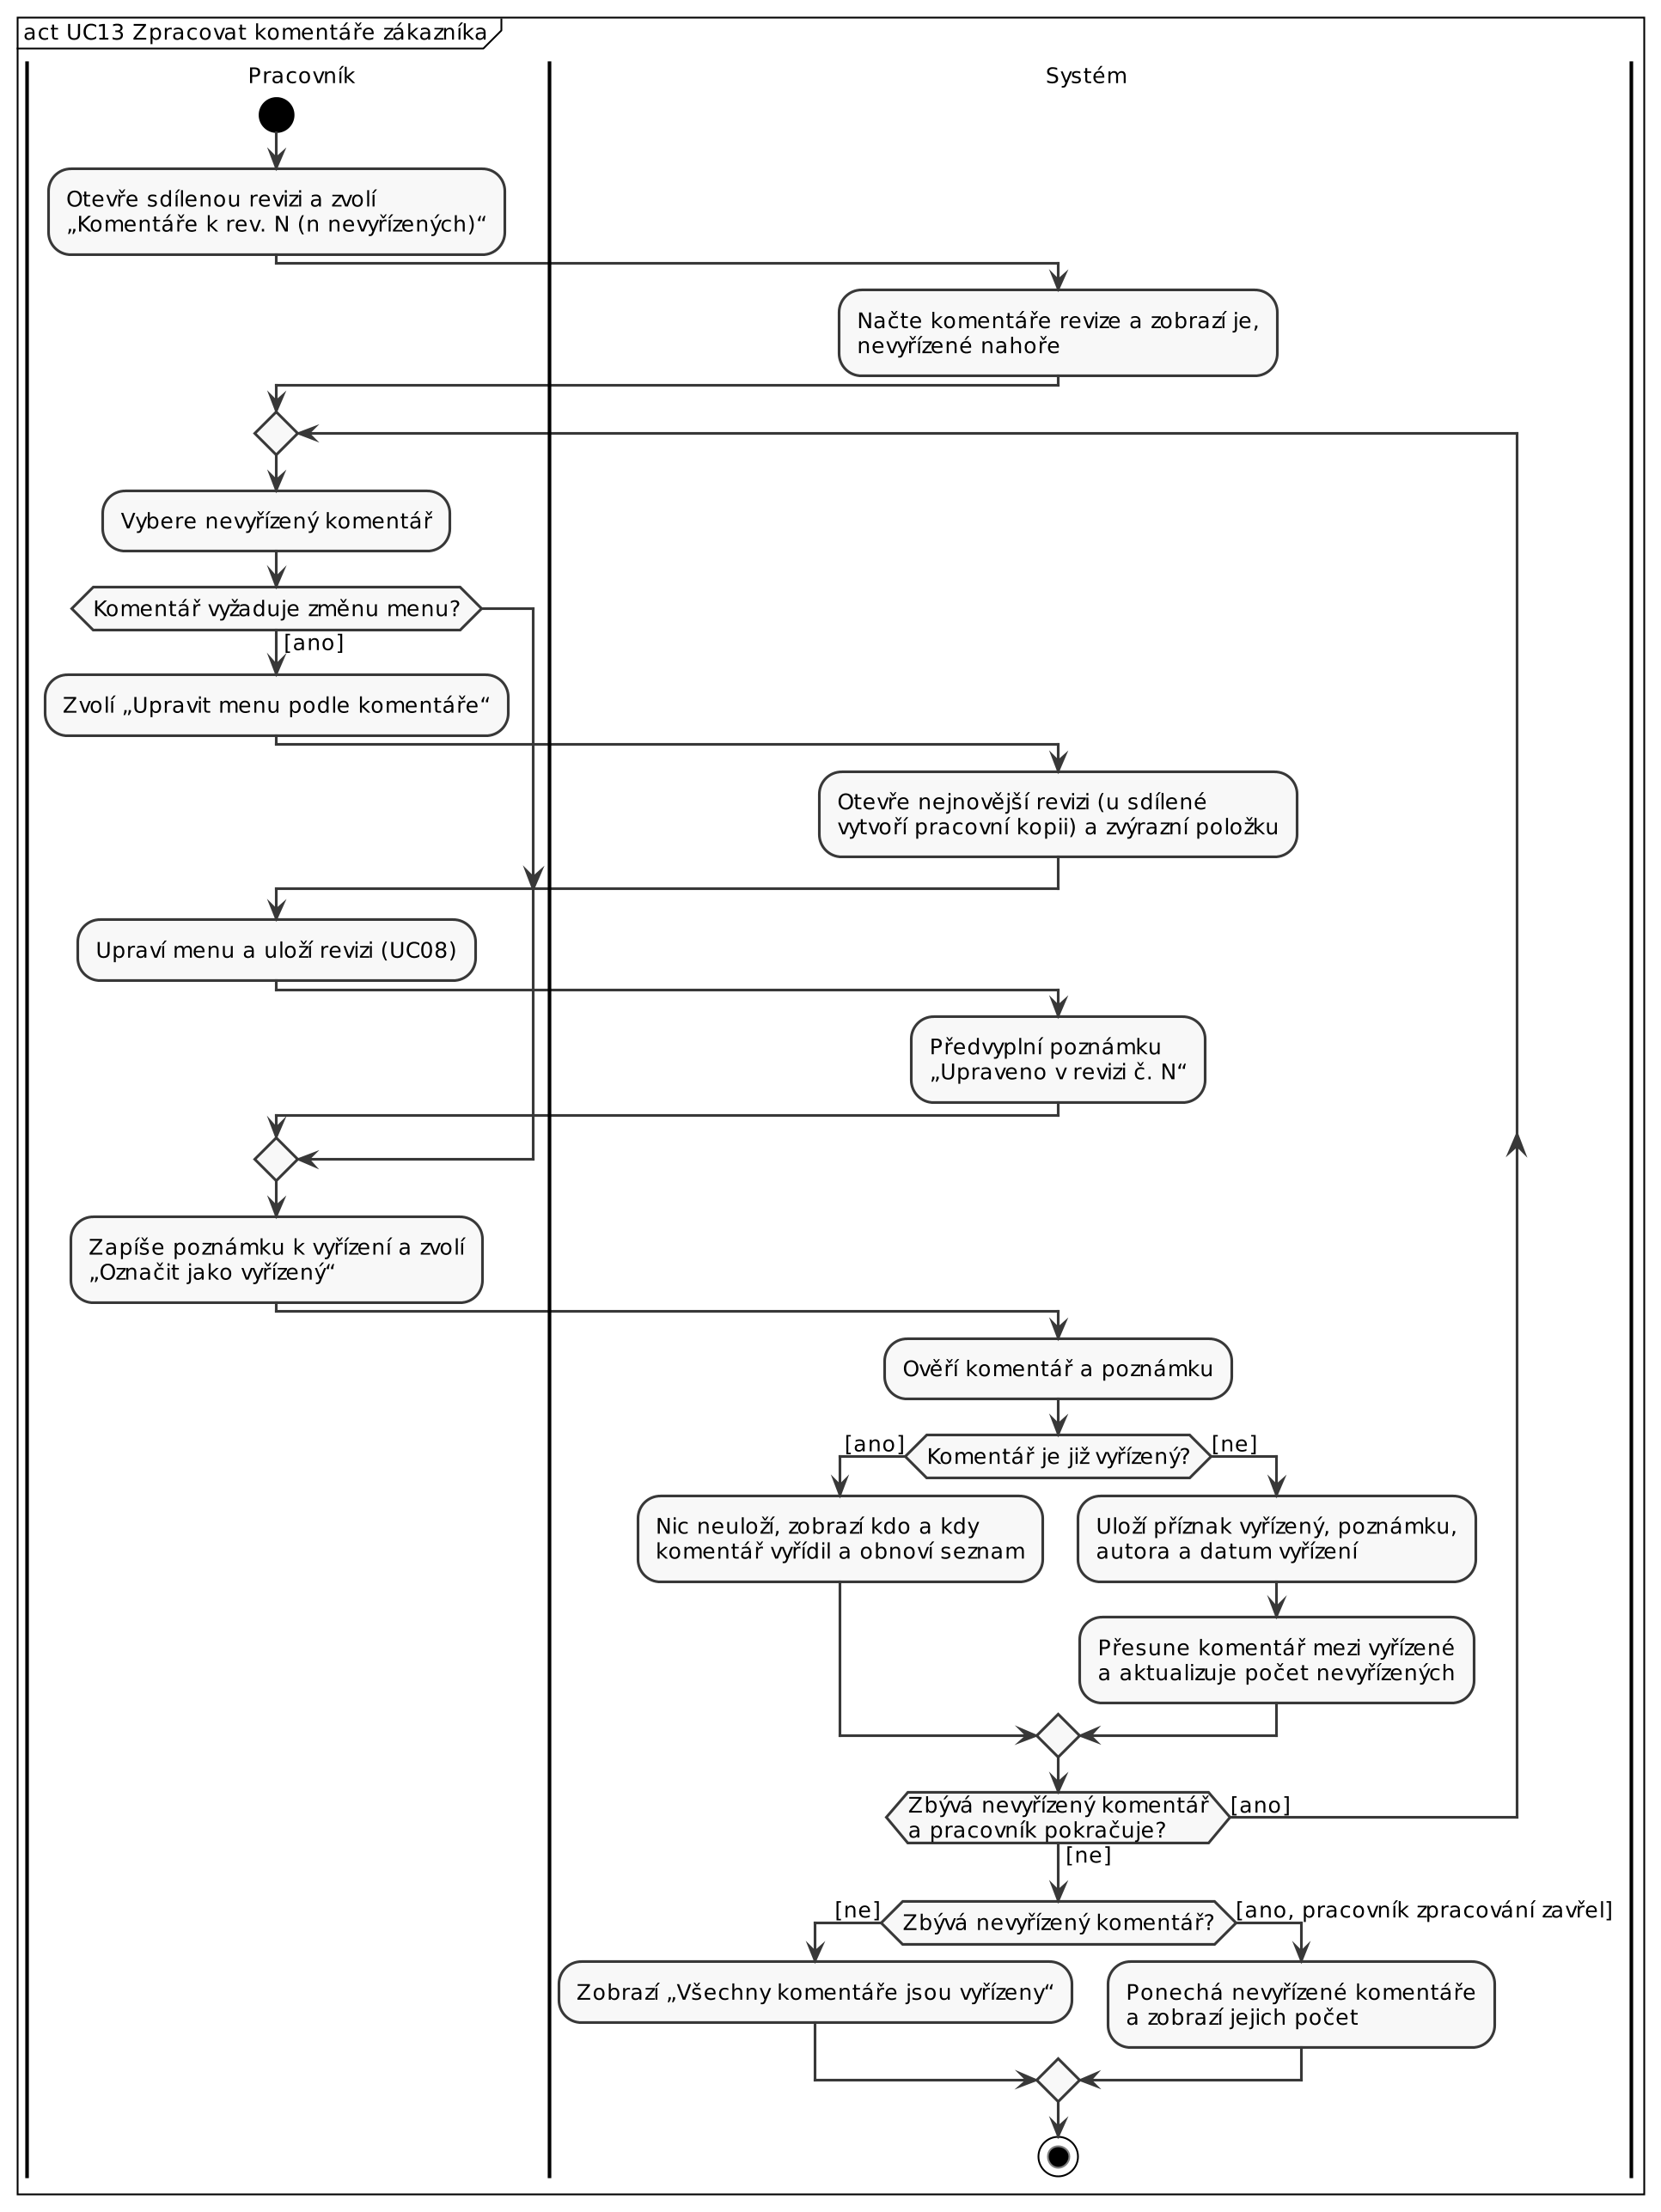
\includegraphics[width=\textwidth,height=0.75\textheight,keepaspectratio]{act-uc13.png}
  \caption{Diagram aktivit UC13 -- Zpracovat komentáře zákazníka}
\end{figure}
\clearpage

% ---------------------------------------------------------------- UC16
\subsubsection{UC16 -- Spravovat uživatele a oprávnění}\label{ucd:16}

\ucpole{Název}
Spravovat uživatele a oprávnění

\ucpole{Textový popis}
Administrátor v administrátorském režimu desktopové aplikace vytváří uživatelské účty pracovníků a manažerů, přiděluje jim role (Pracovník, Manažer, Administrátor), účty deaktivuje a uživateli, který zapomněl heslo, nastaví nové. Systém hlídá jedinečnost uživatelských jmen a nedovolí odebrat posledního aktivního administrátora.

\ucpole{Účastníci případu užití}
Administrátor

\ucpole{Podmínky před spuštěním}
\begin{itemize}[itemsep=0pt]
  \item Uživatel je přihlášen v desktopové aplikaci (\ucref{01}) a má roli Administrátor.
\end{itemize}

\ucpole{Hlavní průběh}
\begin{ucsteps}
  \item \label{uc:16:1}Administrátor přepne aplikaci do administrátorského režimu (\ucref{17}).
  \item \label{uc:16:2}Systém ověří, že uživatel má roli Administrátor, a zobrazí seznam uživatelů s jejich rolemi a stavem. \svc{UserService.findAllUsers()}
  \item \label{uc:16:3}Administrátor zvolí \uv{Nový uživatel}, vyplní uživatelské jméno, celé jméno, e-mail a počáteční heslo a zaškrtne role.
  \item \label{uc:16:4}Systém ověří údaje (povinná pole, formát e-mailu, heslo má alespoň 8 znaků, je vybrána alespoň jedna role) a jedinečnost uživatelského jména. \svc{UserService.createUser()}
  \item \label{uc:16:5}Systém uloží uživatele s hashem hesla a s jeho rolemi a zobrazí jej v seznamu.
  \item \label{uc:16:6}Administrátor vybere existujícího uživatele, změní jeho role, deaktivuje jej nebo mu nastaví nové heslo (například když uživatel heslo zapomněl) a změnu potvrdí.
  \item \label{uc:16:7}Systém ověří, že nové heslo má alespoň 8 znaků a že po změně zůstane v systému alespoň jeden aktivní administrátor, a změnu uloží. Nové heslo uloží jako hash. \svc{UserService.updateUser()}
  \item \label{uc:16:8}Systém aktualizuje seznam uživatelů.
\end{ucsteps}

\ucpole{Alternativní průběh -- údaje jsou neplatné nebo uživatelské jméno již existuje}
\begin{ucalt}
  \item[4.1]\phantomsection\label{uc:16:4.1} Systém zjistí, že některý údaj je neplatný (například chybí e-mail nebo je heslo kratší než 8 znaků), nebo že uživatel se zadaným uživatelským jménem již existuje.
  \item[4.2]\phantomsection\label{uc:16:4.2} Systém uživatele neuloží a zobrazí chybu u příslušného pole.
  \item[4.3]\phantomsection\label{uc:16:4.3} Administrátor údaje opraví a pokračuje krokem \odkaz{uc:16:3}{3}.
\end{ucalt}
Stejně se postupuje, když je nové heslo v kroku \odkaz{uc:16:7}{7} kratší než 8 znaků. Systém změnu neuloží, zobrazí chybu u pole hesla a administrátor pokračuje krokem \odkaz{uc:16:6}{6}.

\ucpole{Alternativní průběh -- odebrání posledního administrátora}
\begin{ucalt}
  \item[7.1]\phantomsection\label{uc:16:7.1} Systém zjistí, že po změně by v systému nezůstal žádný aktivní administrátor.
  \item[7.2]\phantomsection\label{uc:16:7.2} Systém změnu odmítne a nic neuloží.
  \item[7.3]\phantomsection\label{uc:16:7.3} Systém zobrazí zprávu \uv{Systém musí mít alespoň jednoho aktivního administrátora} a vrátí ve formuláři původní hodnoty.
  \item[7.4]\phantomsection\label{uc:16:7.4} Administrátor nejprve přidělí roli Administrátor jinému aktivnímu uživateli (kroky \odkaz{uc:16:6}{6} a \odkaz{uc:16:7}{7}).
  \item[7.5]\phantomsection\label{uc:16:7.5} Administrátor zopakuje původní změnu a systém ji tentokrát uloží a pokračuje se krokem \odkaz{uc:16:8}{8}.
\end{ucalt}

\ucpole{Stav systému po ukončení případu užití}
\begin{itemize}[itemsep=0pt]
  \item V tabulce uživatelů je nový uživatel s hashem hesla a příznakem aktivní. V tabulce přiřazení rolí jsou jeho role.
  \item Upravený uživatel má v databázi nové role, příznak neaktivní nebo nový hash hesla.
  \item V systému existuje alespoň jeden aktivní uživatel s rolí Administrátor.
\end{itemize}

\clearpage
\begin{figure}[H]
  \centering
  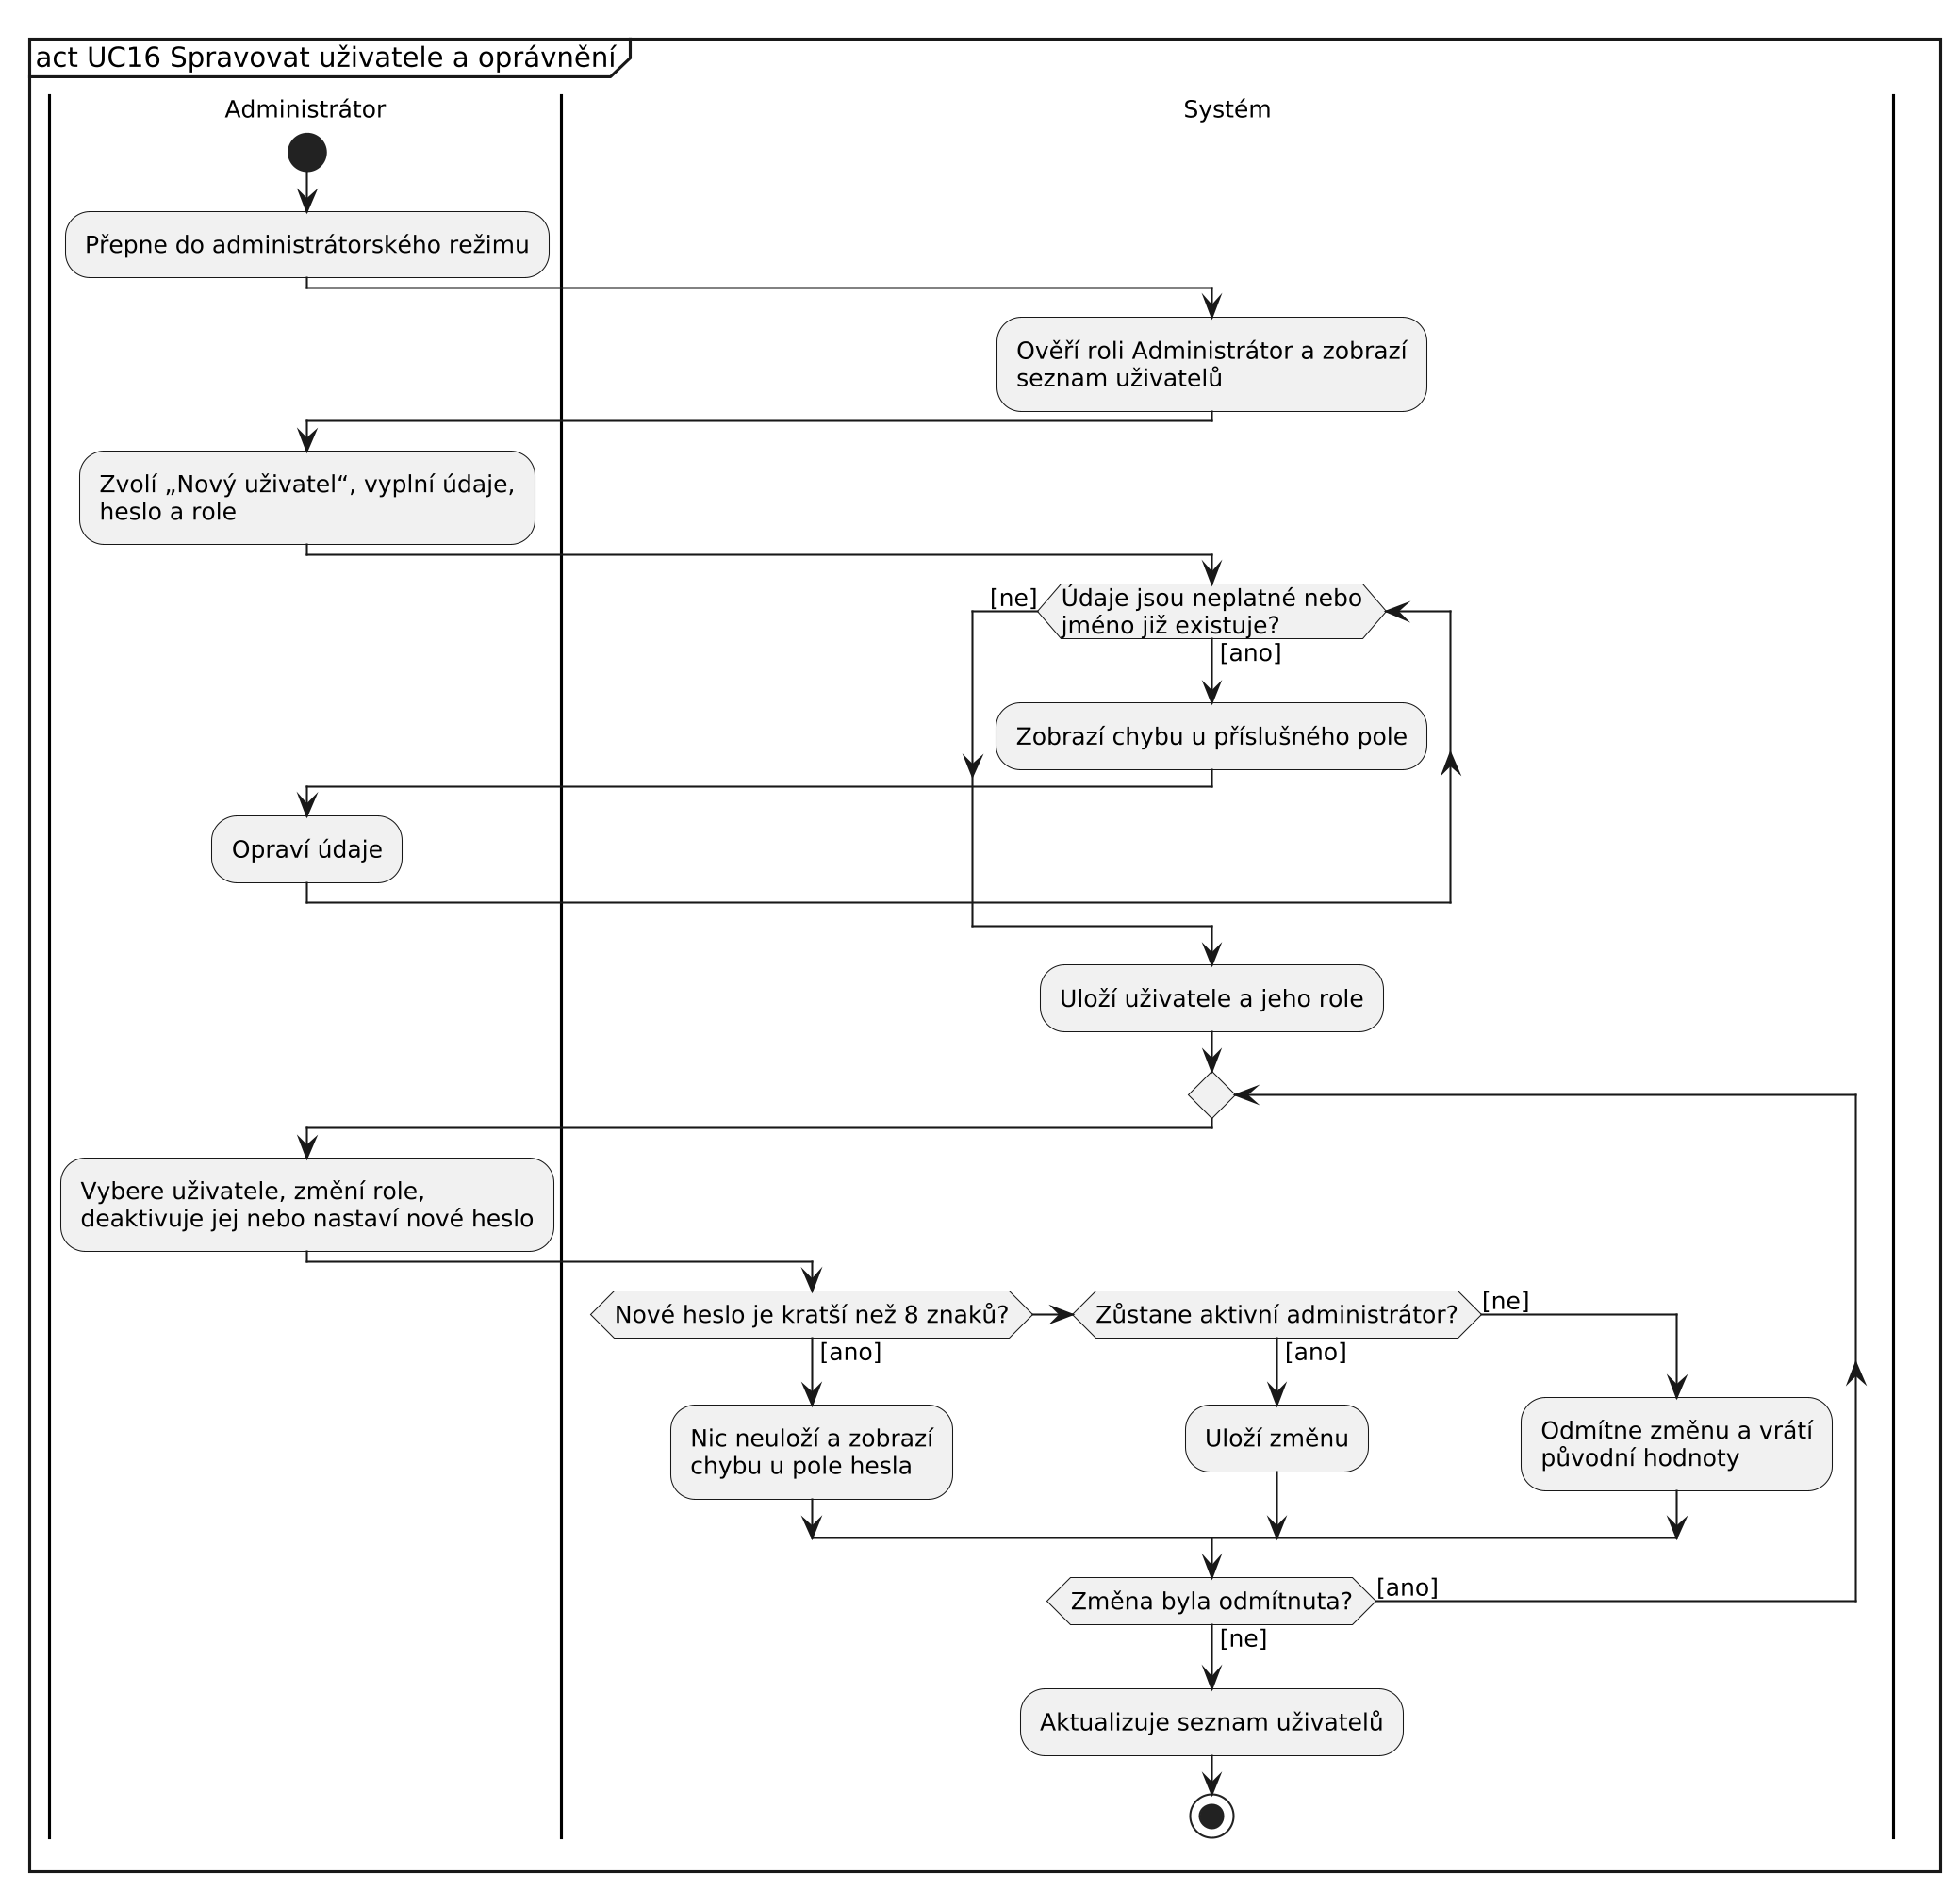
\includegraphics[width=\textwidth,height=0.75\textheight,keepaspectratio]{act-uc16.png}
  \caption{Diagram aktivit UC16 -- Spravovat uživatele a oprávnění}
\end{figure}
\clearpage
